\documentclass{article}

\usepackage[margin=1in]{geometry}
\usepackage{booktabs}
\usepackage{tabularx}
\usepackage{parskip}
\usepackage{longtable}
\usepackage{array}
\usepackage{enumitem}
\usepackage{pdflscape}
\usepackage{graphicx}
\usepackage{float}
\usepackage{hyperref}

\newcommand{\pass}{{\textbf{Pass}}}
\newcommand{\fail}{{\textbf{Fail}}}
\newcommand{\crit}[1]{\textbf{Q#1}}

\newcolumntype{Y}{>{\raggedright\arraybackslash}X}
\setlength{\parskip}{\baselineskip}

\title{CD Fall - Cognitive Walkthrough\\\progname}

\author{\authname}

\date{}

\input{../Comments.text}
\input{../Common.text}

\begin{document}

\maketitle

~\newpage

\pagenumbering{roman}

\begin{table}[!htbp]
\caption{Revision History} \label{TblRevisionHistory}
\begin{tabularx}{\textwidth}{llX}
\toprule
\textbf{Date} & \textbf{Developer(s)} & \textbf{Change}\\
\midrule
2026/11/16 & Ethan McMehen & Completed Everything in the Report \\
2026/11/17 & Ethan McMehen & Applied Minor Changes for Clean up \\
\bottomrule
\end{tabularx}
\end{table}

\newpage

\tableofcontents

\newpage

\pagenumbering{arabic}

% =====================================================================
\section{Introduction}\label{sec:intro}
% =====================================================================

\subsection{What Is a Cognitive Walkthrough?}\label{sec:whatIs}

A cognitive walkthrough is a task-based usability inspection method for evaluating how 
learnable an interface is for a first-time user \cite{nng-overview}. Instead of observing 
real users, a cross-functional group of reviewers steps through each action in a predefined 
task and, at every step, answers a fixed set of questions from the point of view of a 
defined user persona. The goal is to find the parts of an interface that are likely 
to derail a new user.

At each step, the facilitator asks the four questions or variations of the four questions. 
Evaluators discuss four questions \cite{nng-overview, nng-workshop}:
\begin{enumerate}
  \item Will the user try to achieve the right result, that is, understand that this step 
  is needed for their larger goal?
  \item Will the user notice that the correct action is available?
  \item Will the user associate the correct action with the result they are trying to 
  achieve?
  \item After the action is performed, will the user see that progress has been made 
  toward the goal?
\end{enumerate}
If the answer to any question is ``no'', the step is recorded as a \fail{}. The group notes 
why, then continues the analysis as though the step had succeeded so that later steps can 
still be examined \cite{nng-workshop}.

The method was first presented by Lewis and colleagues in 1990 for walk-up-and-use interfaces 
such as kiosks \cite{lewis1990}. The streamlined version most teams use today comes from Wharton 
and colleagues \cite{wharton1994}. The process of the cognitive walkthrough relies on reviewer 
expertise instead of participants and works well on early prototypes. The cognitive walkthrough 
is intended to complement usability testing with real users, not replace it \cite{nng-overview}.

\subsection{Purpose}

This report documents the cognitive walkthrough of the \progname{} gameplay wireframes. Following 
the structure recommended by Nielsen Norman Group, it records the methodology, the people and 
roles involved, and the results, with specific problems identified. A summary of results is also 
included along with the changes planned for the game as a result of the \fail{} recorded in 
walkthrough notes \cite{nng-overview}.

% =====================================================================
\section{Methodology}\label{sec:method}
% =====================================================================

\subsection{\progname{} Cognitive Walkthrough Justification}

\progname{} is a mobile game that prepares the primary end users of children aged 3 to 7, for 
paediatric ophthalmology appointments, with the aim of reducing anxiety and uncertainty 
before the visit \cite{SRS}. Learnability matters more than usual for this audience because 
they are children entering a new and unknown environment. Many of these children cannot read, 
tap imprecisely, have short attention spans, and respond strongly to perceived failure \cite{SRS}. 
Ideally, a first-time user must be able to complete each core task without reading instructions 
or receiving training \cite{SRS}. A game that is confusing to learn could add to the nervousness 
it is meant to reduce.

Therefore, a cognitive walkthrough lets the team check through wireframes if the active approach 
to the game development does not induce further anxiety and nervousness. A cognitive walkthrough 
in particular is useful and necessary to verify this requirement but testing with children requires 
consent and ethics approval that will not be pursued due to the project timing constraints. And testing 
with adults alone cannot demonstrate that the game is usable by children or reduces their anxiety 
\cite{SRS}. The walkthrough is therefore used here to find and remove likely learnability problems 
early, ahead of any child-facing evaluation.

\subsection{Procedure}

The session followed the following cognitive walkthrough format \cite{nng-workshop}:
\begin{enumerate}
  \item \textbf{Briefing.} The facilitator described the purpose, the task, the persona, the roles, 
  and the ground rules.
  \item \textbf{Persona review.} The group discussed what Noah or Sarah already knows and can do 
  before starting.
  \item \textbf{Walkthrough.} The presenter showed each wireframe and asked the evaluators how 
  Noah would act and acted on behalf of evaluators responses. Before the game level, a screen-recording 
  of the level was presented for evaluators to learn the sequence and the narration attached with each 
  scene of the game level. For each step the evaluators answered 
  Q1--Q4, and the notetaker recorded yes or no and the reason for each answer.
  \item \textbf{Determination.} A step was marked \fail{} if any question received a ``no'', and 
  the group continued as though the step had succeeded.
  \item \textbf{Comfort check.} Evaluators also noted any moment that might feel uncomfortable or 
  frightening for the persona because the project's purpose is anxiety reduction.
  \item \textbf{Debrief.} The facilitator summarized the failure points. Design suggestions and 
  the pass/fail determinations that came up were recorded.

\end{enumerate}
The ground rules were to keep discussion on the persona's likely reactions to the design as shown, 
to avoid defending design decisions, and to avoid multitasking \cite{nng-workshop}.

\subsection{Persona, Task, and Action Sequence}

\textbf{Personas:}

The walkthrough was run from the perspective of two personas defined in the SRS \cite{SRS}. 
The SRS personas gave evaluators a shared user context, so they did not rely on imagined users. 
Briefly, the first persona was \textbf{Noah}, a four-year-old 
patient who cannot read independently, is comfortable with basic tapping and dragging, follows short 
spoken instructions and visual demonstrations, and is frustrated by unfamiliar controls that give no 
guidance after a mistake \cite{SRS}. 

The second persona was \textbf{Sarah}, the mother of Noah, who often works 12 to 13-hour shifts, 
balances time with her children and errands on her full days off and noticed Noah's difficulty 
seeing and raised her concerns with the family doctor, leading to referral to an ophthalmologist. 
Before his first eye appointment, she wants to introduce preparation activities on the tablet, 
play alongside him, and help explain anything he does not understand. Evaluators took on one of 
these two personas and judged each step as Noah or Sarah would experience it. 

\textbf{Tasks Evaluated:}
\begin{enumerate}
    \item Enter the game and select the predefined profile to enter the level menu.
    \item Play the Eye Drops game level.
    \item Play the character ``dress-up'' game section with Fits and Eyes catalogues.
\end{enumerate}

The correct action sequence was defined before the session so that the group would not debate 
the path during the walkthrough \cite{nng-workshop}. Table~\ref{tab:sequence} lists it.

\begin{table}[H]
\centering
\caption{Predefined action sequence for the evaluated task.}
\label{tab:sequence}
    \begin{tabularx}{\linewidth}{@{}c Y Y@{}}
    \toprule
    \textbf{Step} & \textbf{Correct Action} & \textbf{Wireframe} \\
    \midrule
    1 & Tap Play & \ref{fig:welcome} \\
    2 & Tap Miguel Profile Picture & \ref{fig:profile} \\
    3 & Tap Either Eye Drops Level or Dress Up (Proceeding with Eye Drops) & \ref{fig:levelmenu} \\
    4 & Tap Green Play Button & \ref{fig:s1}\\
    5 & Tap the Photo of Sam & \ref{fig:s2} \\
    6 & Tap Green Play Button & \ref{fig:s3} \\
    7 & Tap Green Play Button & \ref{fig:s4a} \\
    8 & Tap Green Play Button & \ref{fig:s4b} \\
    9 & Tap Green Play Button & \ref{fig:s5} \\
    10 & Tap Green Play Button & \ref{fig:s6} \\
    11 & Tap Green Play Button & \ref{fig:s7} \\
    12 & Tap the Green Chair & \ref{fig:s9} \\
    13 & Hold the Green Eye Button & \ref{fig:s10a} \\
    14 & Hold the Green Eye Button Longer & \ref{fig:s10b} \\
    15 & Tap Purple Blink Button & \ref{fig:s12a} \\
    16 & Tap Purple Blink Button & \ref{fig:s12b} \\
    17 & Tap Purple Blink Button & \ref{fig:s12c} \\
    18 & Tap Green Play Button & \ref{fig:s13} \\
    19 & Tap Green Menu Button & \ref{fig:final3} \\
    20 & Tap Purple Dress Up Button & \ref{fig:levelmenu} \\
    21 & Scroll the Fits Catalogue & \ref{fig:dressfits} \\
    22 & Tap Buy Button to Buy Fit & \ref{fig:dressfits} \\
    23 & Tap Eyes Button & \ref{fig:dresseyes} \\
    24 & Scroll the Eyes Catalogue & \ref{fig:dresseyes} \\
    25 & Tap Red Back Button & \ref{fig:dresseyes} \\
    \bottomrule
    \end{tabularx}
\end{table}

\subsection{Figma Prototype Evaluation}

The groups evaluated the Figma wireframes shown in Appendix~\ref{sec:figmaPhotos}. The fidelity of a 
prototype limits what a walkthrough can assess \cite{nng-workshop}. The wireframe did not include 
narration or sound effects, but this was accounted for by playing a screen-recording of the game 
to share the narration and the scene animations that would occur during a game level. Minor 
animations were included in the Figma between scene transitions and the final Congratulations scene,
but not to a fully dynamic level that is present in a Unity implemented game \cite{SRS}.

\subsection{Limitations}
Due to the restricted timeline and scope of the capstone project, child-facing evaluation cannot be 
performed due to the required consent and ethics approval clearances. But for further development 
beyond the capstone this remains a necessary step for successful testing practices. \cite{SRS}. The evaluators 
are adults role-playing a child. The persona and the SRS user characteristics reduce the risk of ``fantasy users'' 
\cite{nng-workshop}, but the findings remain predictions about children's behaviour. A walkthrough assesses 
learnability and it does not measure whether the game reduces anxiety. The session used two personas and 3 tasks,
so it does not cover every level or the caregiver flows. The wireframes limit what could be assessed such as narration, 
the clinical script, direct interaction of evaluators with the wireframe, and the game experience within the 
true environment of a home or clinic waiting room \cite{SRS}.

% =====================================================================
\section{People and Roles}\label{sec:people}
% =====================================================================

Ethan performed as the facilitator for all meetings, the full Hindsight team performed the notetaking roles, 
and there was a total of six evaluators with different backgrounds who participated in the review to cover 
several professional perspectives. Table~\ref{tab:session} gives the session details, and the subsections 
below list who filled each role.

\begin{table}[H]
\centering
\caption{Session details.}
\label{tab:session}
\begin{tabularx}{\linewidth}{@{}l l Y@{}}
\toprule
\textbf{Meeting Number} & \textbf{Item} & \textbf{Detail} \\
\midrule
M1 & Date(s) & November 12th \\
& Duration & 30 Minutes \\
& Format & Online \\
& Persona & Noah \\
& Prototype & Figma Wireframe \\
\\
M2 & Date(s) & November 13th \\
& Duration & 30 Minutes \\
& Format & Online \\
& Persona & Noah \\
& Prototype & Figma Wireframe \\
\\
M3 & Date(s) & November 15th \\
& Duration & 30 Minutes \\
& Format & Online \\
& Persona & Sarah \\
& Prototype & Figma Wireframe \\
\bottomrule
\end{tabularx}
\end{table}

\subsection{Facilitators}

The facilitator organizes the session, prepares participants, and keeps the discussion within the purpose and ground rules. 
The facilitator may also act as presenter, who shows the prototype to the group and interacts with it as the persona 
would \cite{nng-workshop}.

\begin{table}[H]
\centering
\begin{tabularx}{\linewidth}{@{}l Y@{}}
\toprule
\textbf{Name} & \textbf{Role and Background} \\
\midrule
Ethan McMehen & Cognitive Walkthrough and Figma Designer, Pursuing Bachelor of Engineering (BEng), McMaster University \\
\bottomrule
\end{tabularx}
\end{table}

\subsection{Evaluators}

Evaluators follow the presenter and answer the four analysis questions for each step from the persona's point of view \cite{nng-workshop}.

\begin{table}[H]
\centering
\begin{tabularx}{\linewidth}{@{}l l Y Y@{}}
\toprule
\textbf{Meeting} & \textbf{Name} & \textbf{Perspective} & \textbf{Background} \\
\midrule
M1 & Emily & Paediatric Clinical Researcher at SickKids Hospital & Honours Bachelor of Health Sciences in BDC (BHSc), McMaster University \\
M2 & Curt & User Interface Expert & Pursuing Bachelor of Engineering (BEng), McMaster University \\
   & Lucas & User Interface Expert & Pursuing Bachelor of Engineering (BEng), McMaster University \\
   & Arjun & User Interface Expert & Pursuing Bachelor of Engineering (BEng), McMaster University \\
M3 & Greg & Parent & Bachelor of Arts (BA English Major), University of Waterloo and Bachelor of Education (BEd), University of Toronto \\
   & Dalila & Parent & Bachelor of Arts (BA Sociology Major), York University and Bachelor of Education (BEd), University of Toronto \\
\bottomrule
\end{tabularx}
\end{table}

\subsection{Notetakers}

The notetaker captures the group's determination and reasoning for each step and later summarizes the findings \cite{nng-workshop}.

\begin{table}[H]
\centering
\begin{tabularx}{\linewidth}{@{}l Y@{}}
\toprule
\textbf{Name} & \textbf{Notes Recorded} \\
\midrule
Ethan McMehen & Ethan\_CW\_Nov12\_Notes.md \\
Jake Finlay & Jake\_CW\_Nov13\_Notes.md \\
Ahsan Muzammil & Ahsan\_CW\_Nov13\_Notes.md \\
Jackson Beach & Jackson\_CW\_Nov15\_Notes.md \\
\bottomrule
\end{tabularx}
\end{table}

% =====================================================================
\section{Results}\label{sec:results}
% =====================================================================

\subsection{Overview}

Table~\ref{tab:results} gives the outcome for each of the 25 steps in the predefined action sequence 
(Table~\ref{tab:sequence}). A step is marked \fail{} if the evaluators answered ``no'' to any of the 
four analysis questions (Section~\ref{sec:whatIs}) in any session, and the question it failed on is listed. Sessions 
are referred to as M1 to M3 (Table~\ref{tab:session}).

11 of the 25 steps failed, 14 passed. Step 22 failed under \crit{1}. Eight failures were on \crit{2},
meaning the child may not notice the correct action: choosing a profile (step 2), tapping Sam (5) and the chair (12), 
blinking (15 to 17), the end-of-game button (19), and the Back button (25). Steps 13 and 14, holding the green eye 
button, failed on \crit{3}, and step 14 also on \crit{4}. The blink interaction itself was judged intuitive in one 
session, but two sessions said children need explicit instruction to use it. Detailed findings follow the table.

\subsection{Results by Step}

{\small
\begin{longtable}{@{}>{\centering\arraybackslash}p{0.9cm} >{\raggedright\arraybackslash}p{4.0cm} >{\centering\arraybackslash}p{1.7cm} >{\centering\arraybackslash}p{1.4cm} >{\raggedright\arraybackslash}p{\dimexpr\linewidth-8.0cm-8\tabcolsep\relax}@{}}
\caption{Results for Each Action}
\label{tab:results}\\
\toprule
\textbf{Step} & \textbf{Correct action} & \textbf{Outcome} & \textbf{Q} & \textbf{Reason} \\
\midrule
\endfirsthead
\multicolumn{5}{@{}l}{\small\textit{Table~\thetable{} (continued)}}\\
\toprule
\textbf{Step} & \textbf{Correct action} & \textbf{Outcome} & \textbf{Q} & \textbf{Reason} \\
\midrule
\endhead
\midrule
\multicolumn{5}{r@{}}{\small\textit{Continued on next page}}\\
\endfoot
\bottomrule
\endlastfoot

1 & Tap Play & \pass & --- &
  The Play button draws the eye (M2, M3). Curious children may tap other things first, but the green button makes sense 
  once direction is clear (M1). The waving animation may distract or mislead (M2). \\
2 & Tap Miguel Profile Picture & \fail & \crit{2} &
  Non-readers may not know to press their character's picture and may press the green Home button instead (M2). Miguel 
  is an appealing choice because he is a person (M1). \\
3 & Tap Eye Drops Level (or Dress Up) & \pass & --- &
  The menu makes sense (M1), and the green and large purple buttons draw attention (M2). Children are likely to try 
  Dress Up first (M1, M3), which is allowed. Non-readers may need help (M3). \\
4 & Tap Green Play Button & \pass & --- &
  Evaluators identified Play as the way to start the level (M3), and the green button draws attention (M2). \\
5 & Tap the Photo of Sam & \fail & \crit{2} &
  It is not obvious that Sam is tappable. Children may press the volume button or the green button instead (M2). 
  Evaluators recommended a glow or pulse on Sam (M1, M3), and the progress bar cuts off the yellow arrow (M2). \\
6 & Tap Green Play Button & \pass & --- &
  The pulsating green button draws attention and shows how to progress (M1, M3). \\
7 & Tap Green Play Button & \pass & --- & As step 6. \\
8 & Tap Green Play Button & \pass & --- & As step 6. \\
9 & Tap Green Play Button & \pass & --- & As step 6. \\
10 & Tap Green Play Button & \pass & --- & As step 6. \\
11 & Tap Green Play Button & \pass & --- & As step 6. \\
12 & Tap the Green Chair & \fail & \crit{2} &
  The chair needs a stronger indicator, such as a glow or animation, together with explicit narration like ``Tap 
  the green chair'' (M1, M3). M2 felt the glowing arrow would probably be enough. \\
13 & Hold the Green Eye Button & \fail & \crit{3} &
  The button looks like a tap button and only the voiceover says to hold, so children may spam it (M2). Parents are 
  expected to need to help, and Dr.~Iris should repeat ``hold the button'' (M1, M3). \\
14 & Hold the Green Eye Button Longer & \fail & \crit{3}, \crit{4} &
  Same problem as step 13. The progress bar helps parents see how long to hold (M3), but children may ignore it (M1, M3) 
  or mistake it for a button (M2), so they may not see progress. \\
15 & Tap Purple Blink Button & \fail & \crit{2} &
  Pressing to blink is intuitive (M2), but children need explicit narration and a visible cue to know to press it, 
  otherwise they may not catch it (M1, M3). \\
16 & Tap Purple Blink Button & \fail & \crit{2} & As step 15. \\
17 & Tap Purple Blink Button & \fail & \crit{2} & As step 15. \\
18 & Tap Green Play Button & \pass & --- &
  The reward and congratulations scenes make sense, and success is clear (M1, M2), so \crit{4} is satisfied. \\
19 & Tap Green Menu Button & \fail & \crit{2} &
  It was unclear which button to press after the game ended (M2). The green Menu looks like the green forward arrow 
  (M2, PoC), Play could mean next level or replay (M3), and adults found Home and Menu unclear (M3). \\
20 & Tap Purple Dress Up Button & \pass & --- &
  The purple button and t-shirt icon draw interest (M2, M3), and with guidance 3 to 4 year olds would press it (M1). \\
21 & Scroll the Fits Catalogue & \pass & --- &
  The layout is intuitive, and children are expected to try every choice (M1, M2, M3). \\
22 & Buy an Outfit & \fail & \crit{1} &
  Children may not understand why they should buy the outfit. Money is confusing for ages 3 to 4, and children may not 
  know what coins do (M1, M2, M3). A 4-year-old would likely just pick the outfit they like (M3). The buy button itself 
  makes sense with guidance (M1). \\
23 & Tap Eyes Button & \pass & --- &
  Switching sections is clear (M2), and the customization menus are intuitive (M3). \\
24 & Scroll the Eyes Catalogue & \pass & --- &
  Children want to try every option (M1, M3). \\
25 & Tap Red Back Button & \fail & \crit{2} &
  M1 found the red button intriguing to press, but children may not know to press Back and could get stuck on the customization 
  screen (M2). Parents would press Done first, and Done and Back seem redundant (M3). \\
\end{longtable}
}

\subsection{Detailed Findings}

\textbf{F1. Hold the Green Eye Button (steps 13--14) \fail{}, \crit{3}, \crit{4}.}
All three sessions raised this as an issue. The button looks pressable but only the voiceover says it must be held, 
so children may tap repeatedly instead (M2). Parents would need to help, and Dr.~Iris should repeat the specific 
instruction to hold (M1, M3). Because children in this age range react strongly to perceived failure \cite{SRS}, a 
failed attempt could add to their nervousness. Additionally, in M2, feedback on the Proof of Concept proposed that 
holding keeps the eyes open and advances the yellow progress wheel. Releasing stops the wheel and closes the eyelids 
slowly, with a black screen only when the eyes are fully closed. Pressing again reopens the eyes immediately, and 
there is no failure state or reset.

\textbf{F2. The Purple Blink Button (steps 15--17) \fail{}, \crit{2}.}
Sessions disagreed. M2 found pressing to blink intuitive, but M1 and M3 said children need explicit instruction, otherwise 
they and their parents may not catch it. The interaction itself is understood once prompted, so the problem is noticing when 
to use it.

\textbf{F3. Targets that are not Obvious (steps 2, 5, 12, 25) \fail{}, \crit{2}.}
Four steps share one cause: the intended target is not noticeable enough for a child who cannot read. Evaluators recommended 
a glow or pulse on Sam and the chair (M1, M3), explicit narration (M1, M3), and noted that the progress bar competes with 
the arrow cue (M2, PoC). Feedback for the PoC from M2 also proposed a gentle pulse on the expected element when the child is 
inactive to refocus the attention to the interactive element.

\textbf{F4. End of Game (steps 18--19).}
The reward and congratulations scenes make success clear (step 18, \crit{4}). But Step 19 fails on \crit{2}: the green Menu 
looks like the forward arrow, the meaning of Play is unclear, and adults found Home and Menu hard to tell apart (M2, M3, PoC).

\textbf{F5. Forward Navigation and Use of a Consistent Colour.}
Evaluators asked for an always-available forward button that glows after a wrong tap (M1, M2). M3 liked consistent green buttons, 
while M2 and the PoC feedback warn that a green Menu button is confused with ``go''. The common conclusion was to reserve 
green for forward or start actions only (M1, M2, M3).

\textbf{F6. Progress Bar.}
Children may not notice the bar (M1) or may think it is a button (M2), and it covers the yellow arrow on Sam's screen (M2, PoC). 
Parents found it useful and clearly placed (M3).

\textbf{F7. Currency and Rewards (Dress Up) \fail{}, \crit{1}.}
All three sessions found money confusing for young children. Evaluators suggested calling rewards ``prizes'' or using collectible 
stars, and M3 suggested leaving purchasing out for about four-year-olds.

\textbf{F8. Content Observations.}
Children are literal and may assume both eyes are treated, so animations should show both (M3). Evaluators disagreed on whether 
children would understand that the drops cause discomfort: M1 thought they might, M2 was unsure, and noted that the screen dimming 
signals that something is happening. All evaluators agreed that fear or severe discomfort was not shown.

\textbf{F9. General Successes.}
Evaluators praised the animations, the script language, the glowing description over narration, the pupil-enlargement explanation, 
the congratulations scene, and the character layout. Nothing felt uncomfortable (M2).

% =====================================================================
\section{Planned Changes}\label{sec:planned}
% =====================================================================

Table~\ref{tab:changes} converts each finding into a planned change.

{\small
\begin{longtable}{@{}>{\raggedright\arraybackslash}p{0.9cm} >{\raggedright\arraybackslash}p{1.0cm} >{\raggedright\arraybackslash}p{\dimexpr\linewidth-6.2cm-6\tabcolsep\relax}@{}}
\caption{Planned interface changes.}
\label{tab:changes}\\
\toprule
\textbf{ID} & \textbf{From} & \textbf{Planned Change} \\
\midrule
\endfirsthead
\toprule
\textbf{ID} & \textbf{From} & \textbf{Planned Change} \\
\midrule
\endhead
\bottomrule
\endlastfoot
C1 & F1 &
  Make the hold requirement visible and narrated. Use the gradual-eyelid design: holding advances the progress, releasing 
  stops it and closes the eyes slowly, black only when fully closed, with no failure state. \\
C2 & F2 &
  Add explicit narration (``tap the purple blink button'') and a pulsing cue or glowing effect on the blink button each time 
  it is needed. Or consider keeping the button green to signify next with the blink icon. \\
C3 & F3 &
  Add a glow or pulse on the intended target (Sam, chair, profile picture, Back or Done) with explicit narration. Pulse the 
  expected target gently after inactivity, and stop when the child touches it. Consider also including narration through the 
  game pages as a guide as well and not just for the levels themselves. \\
C4 & F4 &
  On the end-of-game screen, give a Play Next and Menu Level option with distinct colours. Play Next should be green to maintain the 
  colour consistency of progression. Using the distinct colours and icons, make the recommended action 
  most prominent, and keep a clear stop control. \\
C5 & F5 &
  Always show a forward button in one consistent place that glows after a wrong tap. Use green only for forward or start 
  actions, and give the Menu a different colour and a home or menu icon. \\
C6 & F6 &
  Simplify the progress bar from the child view or move it to a caregiver view for assistance, and keep arrow cues uncovered. \\
C7 & F7 &
  Replace money and coin wording with prizes or collectible stars, and consider removing purchasing for the youngest 
  children. This change will most likely require a change in rewards requirements in the SRS to reflect the feedback 
  obtained. \\
C8 & F8 &
  Show the drops going into both eyes, and review the discomfort cue so children understand a sensation is coming. \\
C9 & F9 &
  Keep the animations, script wording, glowing description over narration, congratulations scene, and character layout. 
  Review the waving title animation. Ensure instructions are literal, as this was a positive for clear scenes. \\
\end{longtable}
}

These changes will contain issues created in GitHub to track the development and attention to these new implementations and changes. 
GitHub issues will be reviewed and resolved by team members to ensure the changes have met the standards of the SRS requirements and 
the feedback provided by evaluators from the cognitive walkthrough.

\newpage
% =====================================================================
\section{Appendices}
% =====================================================================
% =====================================================================
\subsection{Appendix A: Figma Prototype}
\label{sec:figmaPhotos}
% =====================================================================

The cognitive walkthrough wireframe was developed in Figma. The prototype can be directly accessed through this 
\href{https://www.figma.com/proto/IBdPBjcaoQjUY02BwWSvpv/EyeCanDo-Cognitive-Walkthrough?node-id=7-2&t=wh38lXowwpUC86ZR-1&scaling=scale-down&content-scaling=fixed&page-id=0%3A1&starting-point-node-id=7%3A2}{Figma link}. 
Photographs have also been included below for viewing the prototype statically:

\begin{figure}[H]
    \centering
    \caption{Welcome Scene}
    \label{fig:welcome}
    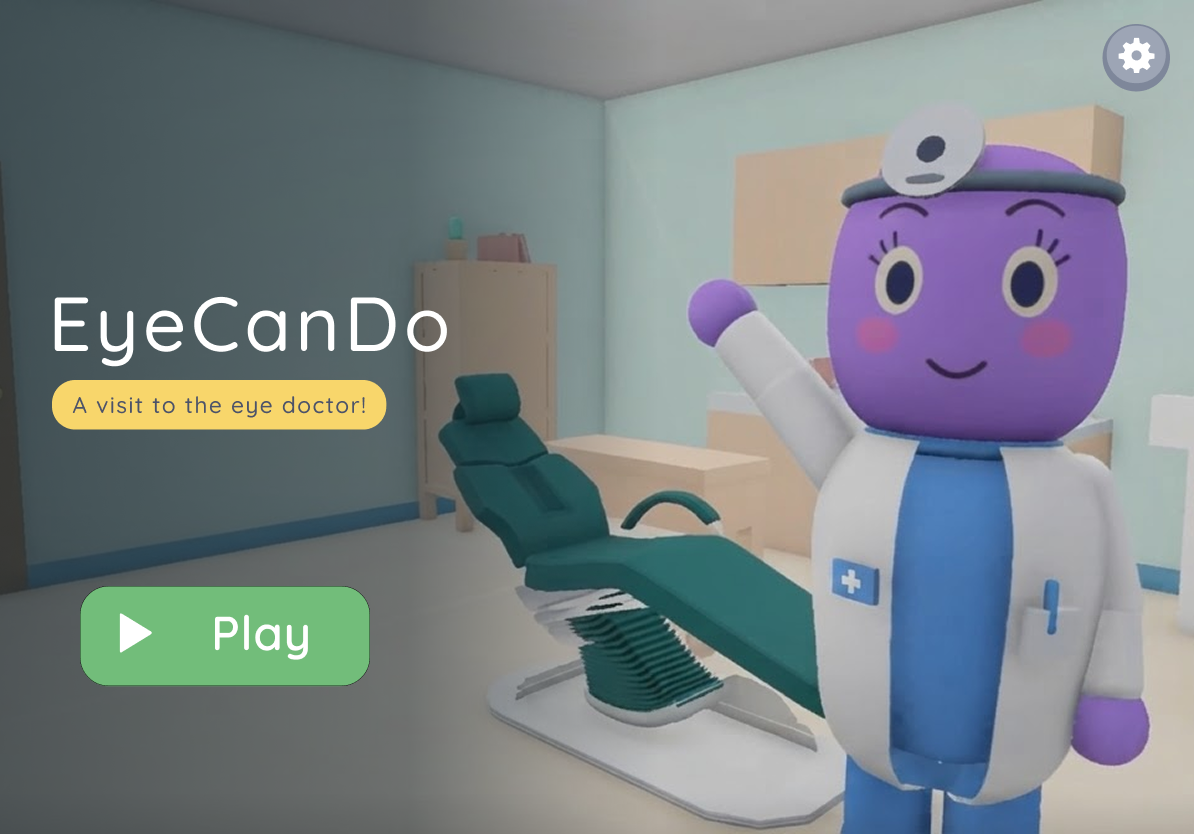
\includegraphics[width=0.8\textwidth]{EyeCanDoCW/EyeCanDoWelcome.png}
\end{figure}

\begin{figure}[H]
    \centering
    \caption{Profile Selection Scene}
    \label{fig:profile}
    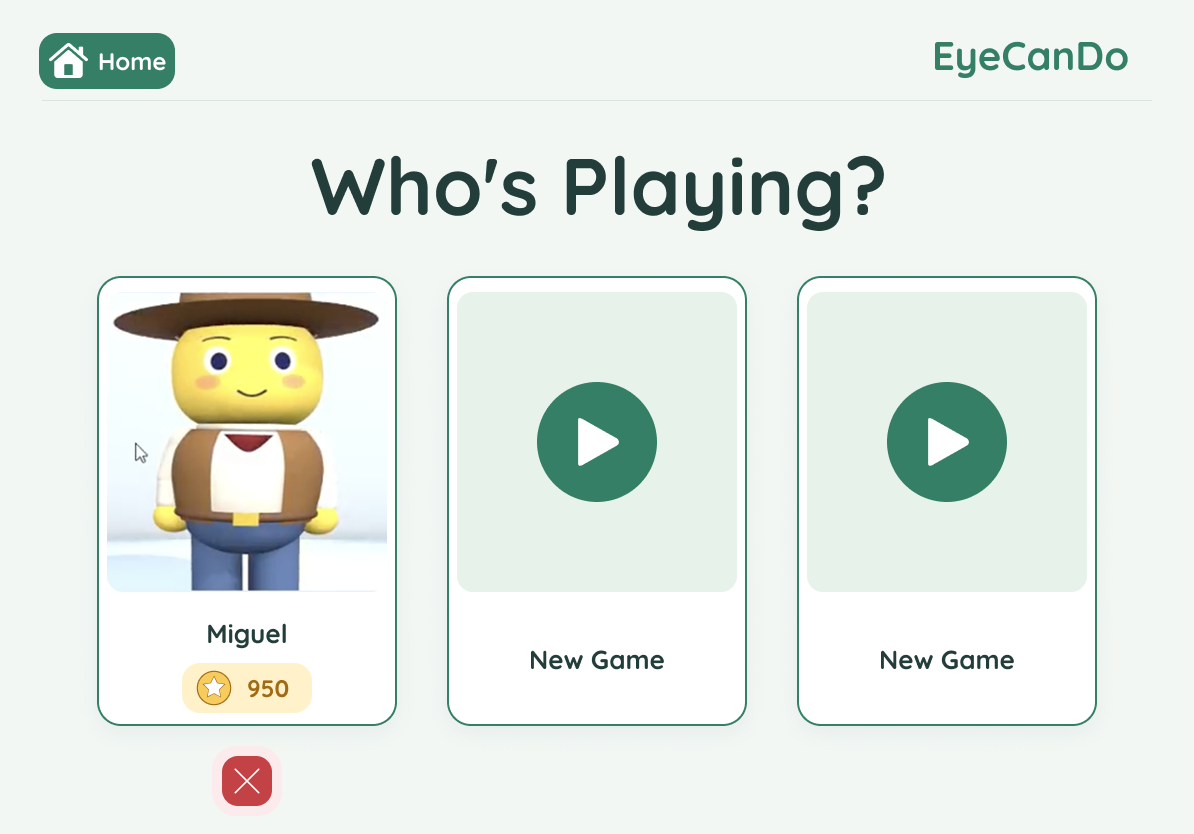
\includegraphics[width=0.8\textwidth]{EyeCanDoCW/ProfileSelection.png}
\end{figure}

\begin{figure}[H]
    \centering
    \caption{Level Menu Scene}
    \label{fig:levelmenu}
    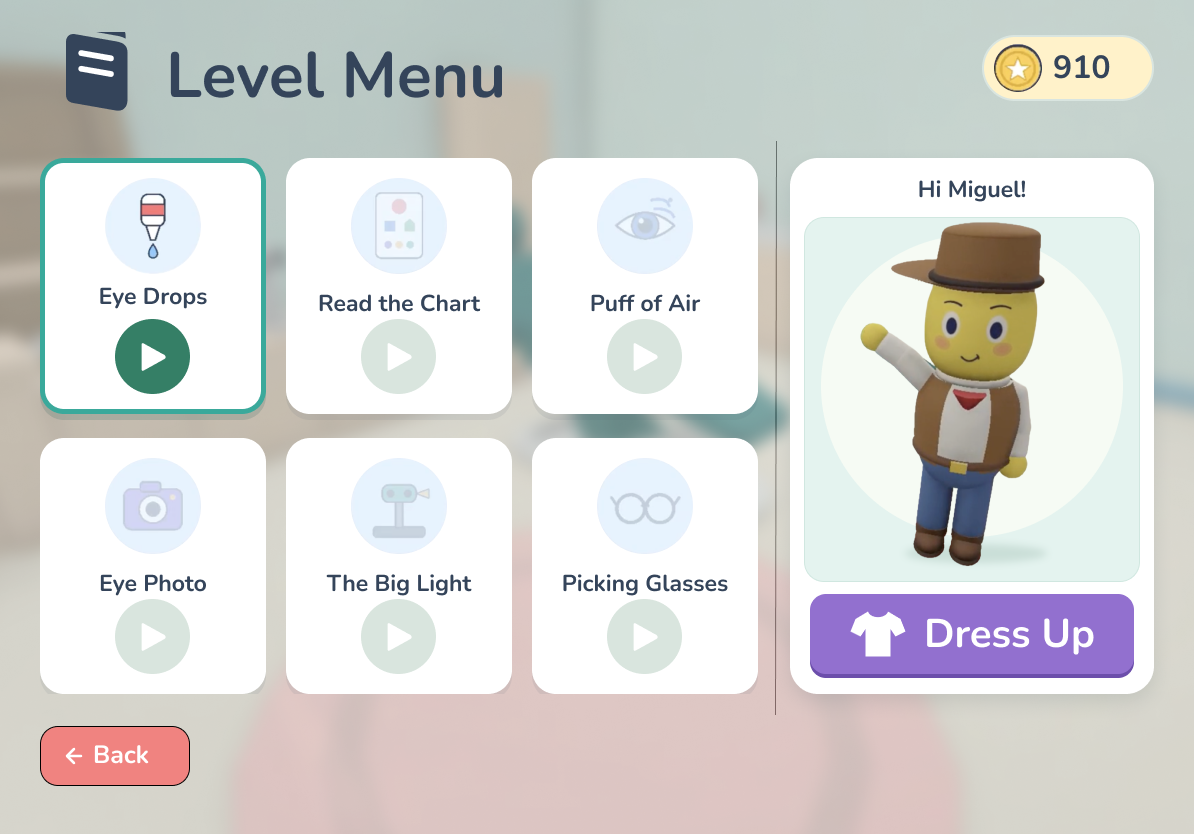
\includegraphics[width=0.8\textwidth]{EyeCanDoCW/Level Menu.png}
\end{figure}

\begin{figure}[H]
    \centering
    \caption{First Scene}
    \label{fig:s1}
    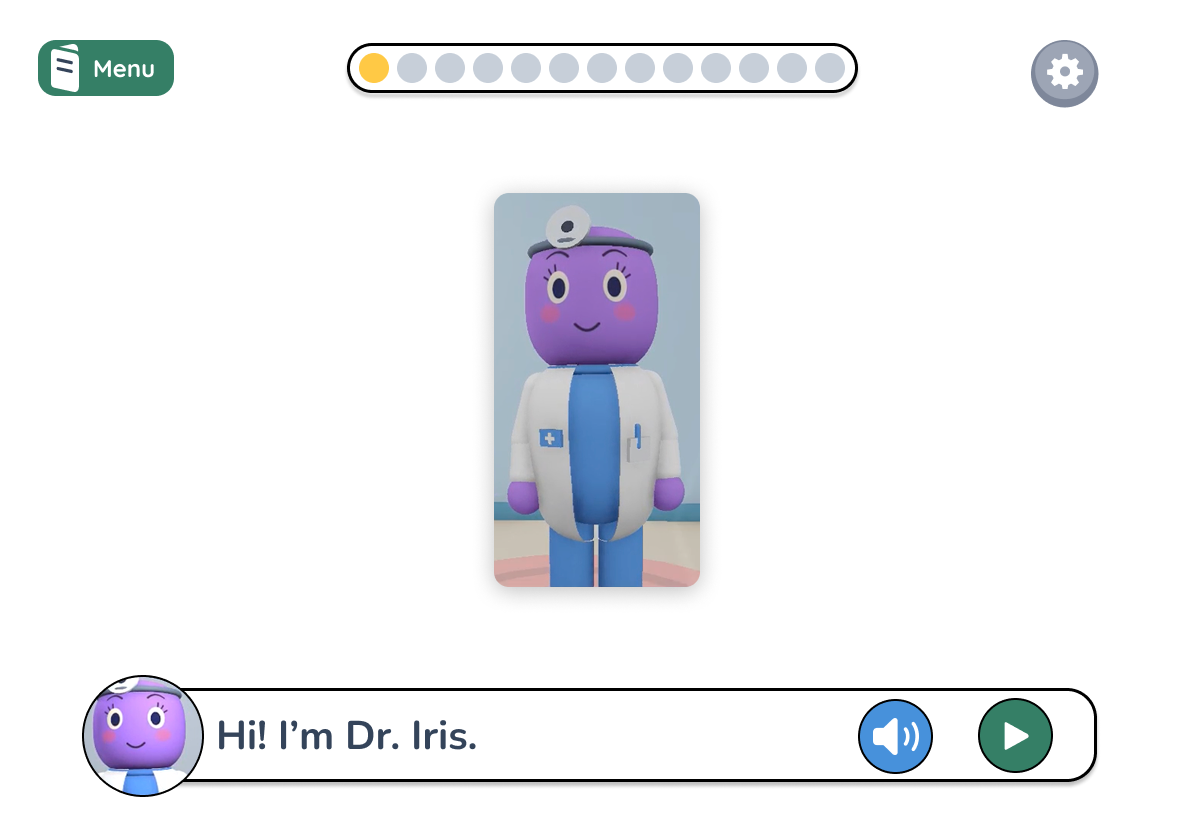
\includegraphics[width=0.8\textwidth]{EyeCanDoCW/First Scene.png}
\end{figure}

\begin{figure}[H]
    \centering
    \caption{Second Scene}
    \label{fig:s2}
    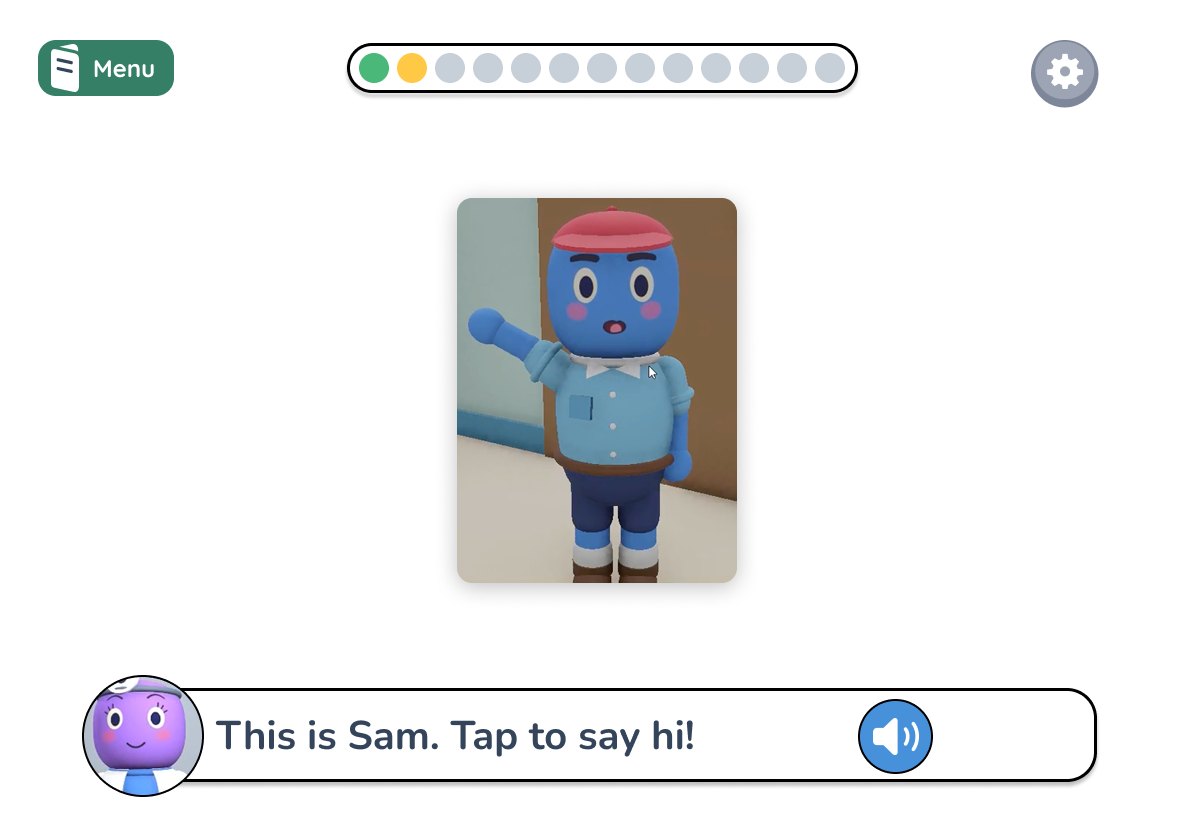
\includegraphics[width=0.8\textwidth]{EyeCanDoCW/Second Scene.png}
\end{figure}

\begin{figure}[H]
    \centering
    \caption{Third Scene}
    \label{fig:s3}
    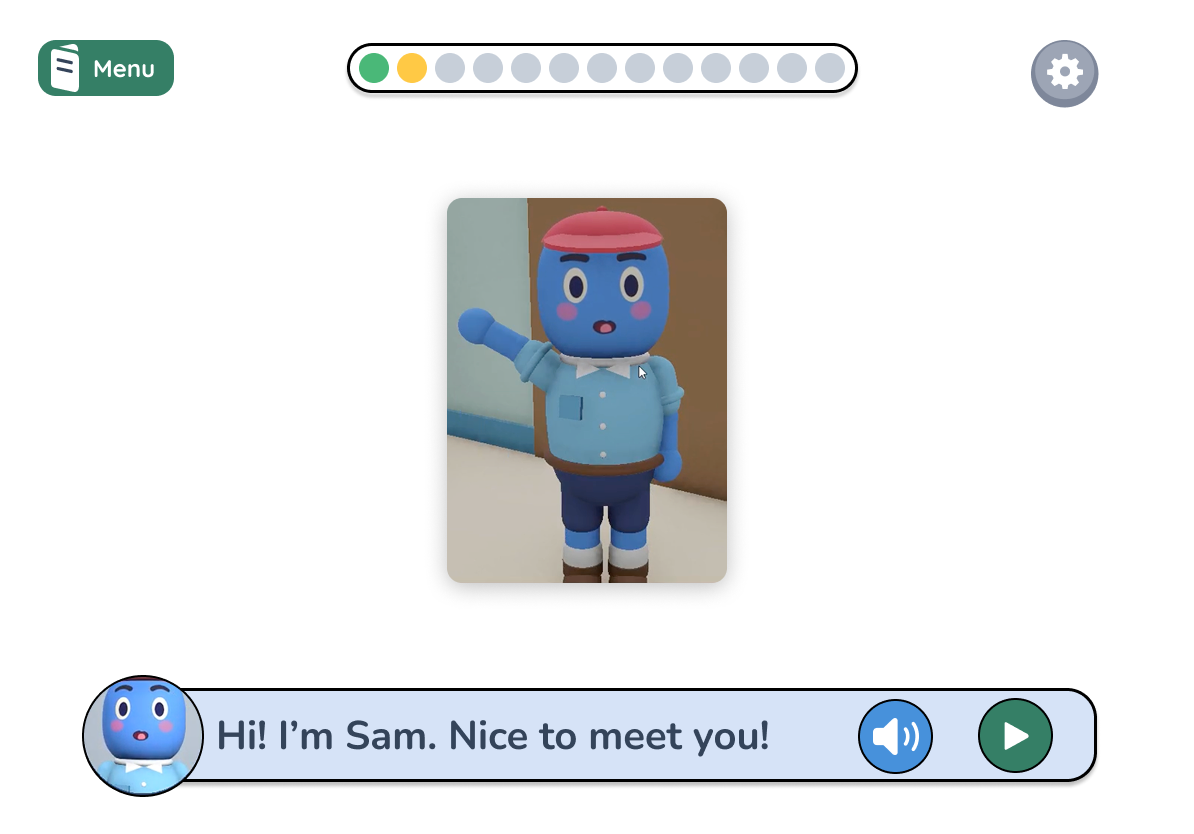
\includegraphics[width=0.8\textwidth]{EyeCanDoCW/Third Scene.png}
\end{figure}

\begin{figure}[H]
    \centering
    \caption{Fourth Scene}
    \label{fig:s4a}
    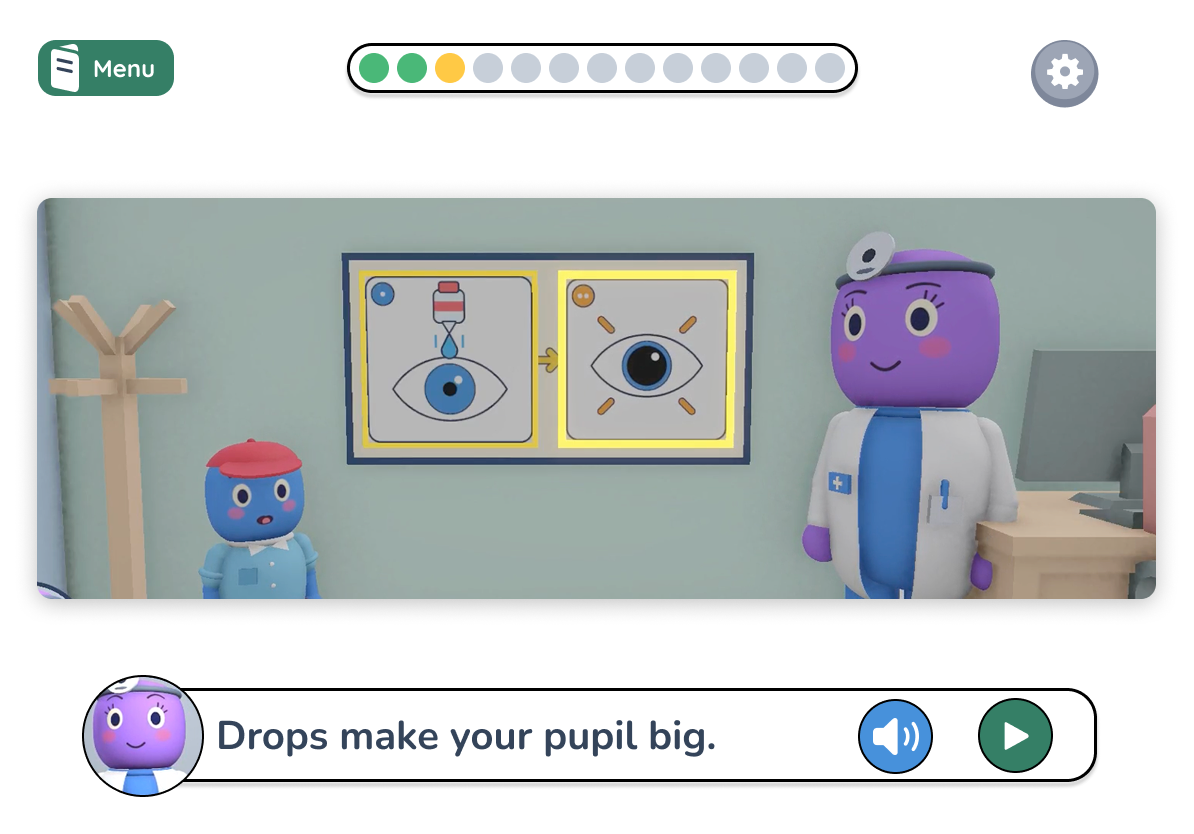
\includegraphics[width=0.8\textwidth]{EyeCanDoCW/Fourth Scene.png}
\end{figure}

\begin{figure}[H]
    \centering
    \caption{Fourth Scene 2}
    \label{fig:s4b}
    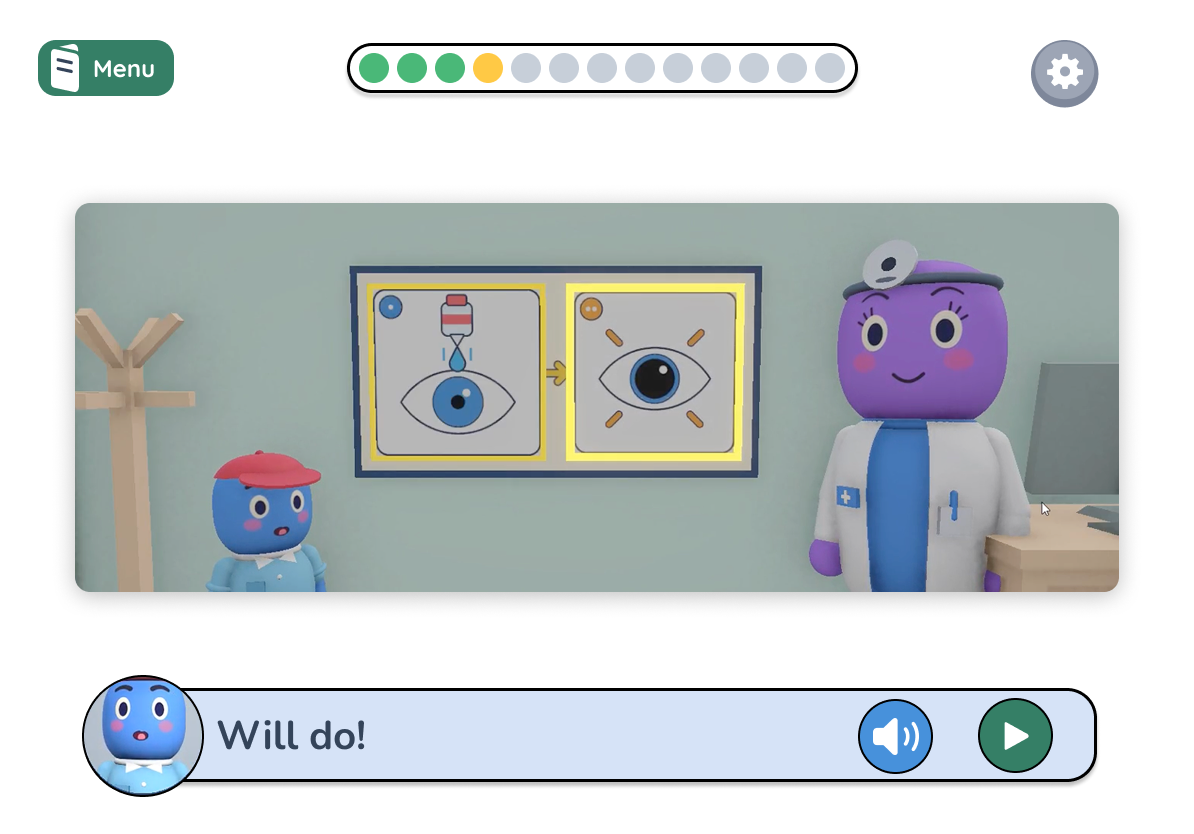
\includegraphics[width=0.8\textwidth]{EyeCanDoCW/Fourth Scene 2.png}
\end{figure}

\begin{figure}[H]
    \centering
    \caption{Fifth Scene}
    \label{fig:s5}
    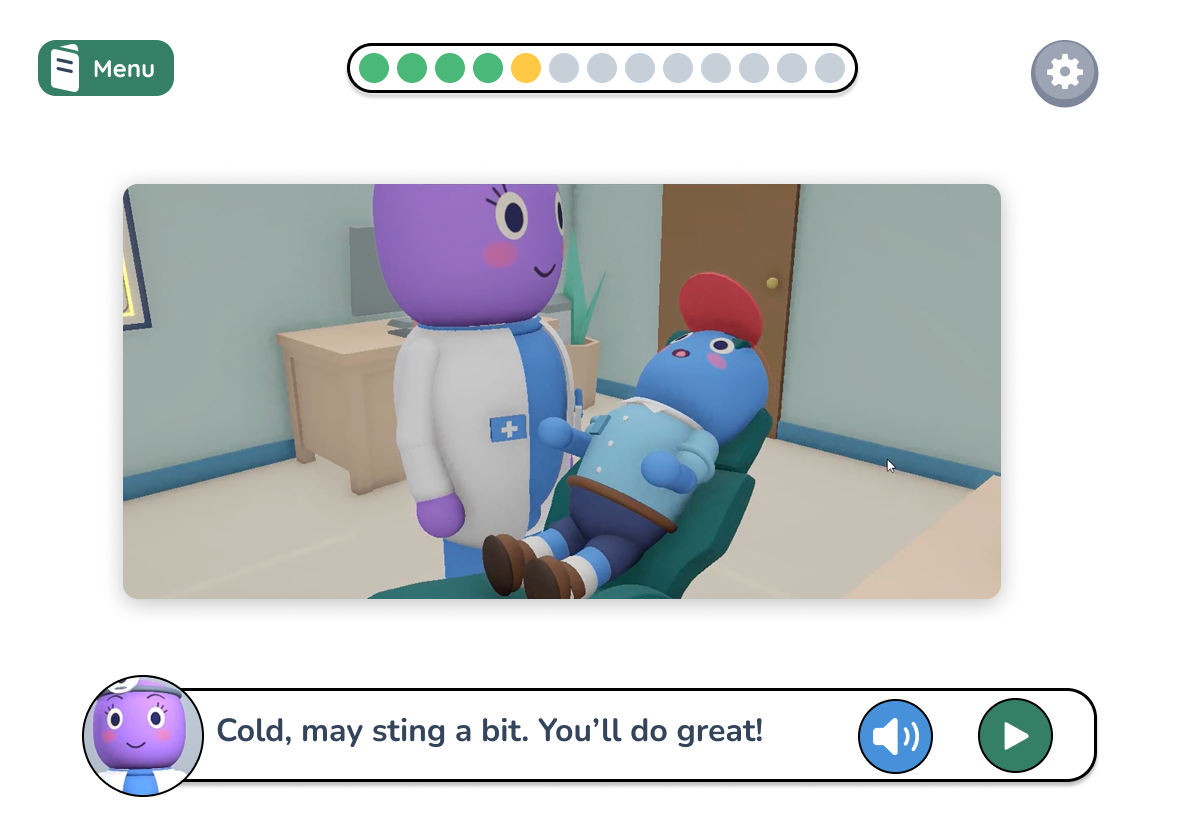
\includegraphics[width=0.8\textwidth]{EyeCanDoCW/Fifth Scene.png}
\end{figure}

\begin{figure}[H]
    \centering
    \caption{Sixth Scene}
    \label{fig:s6}
    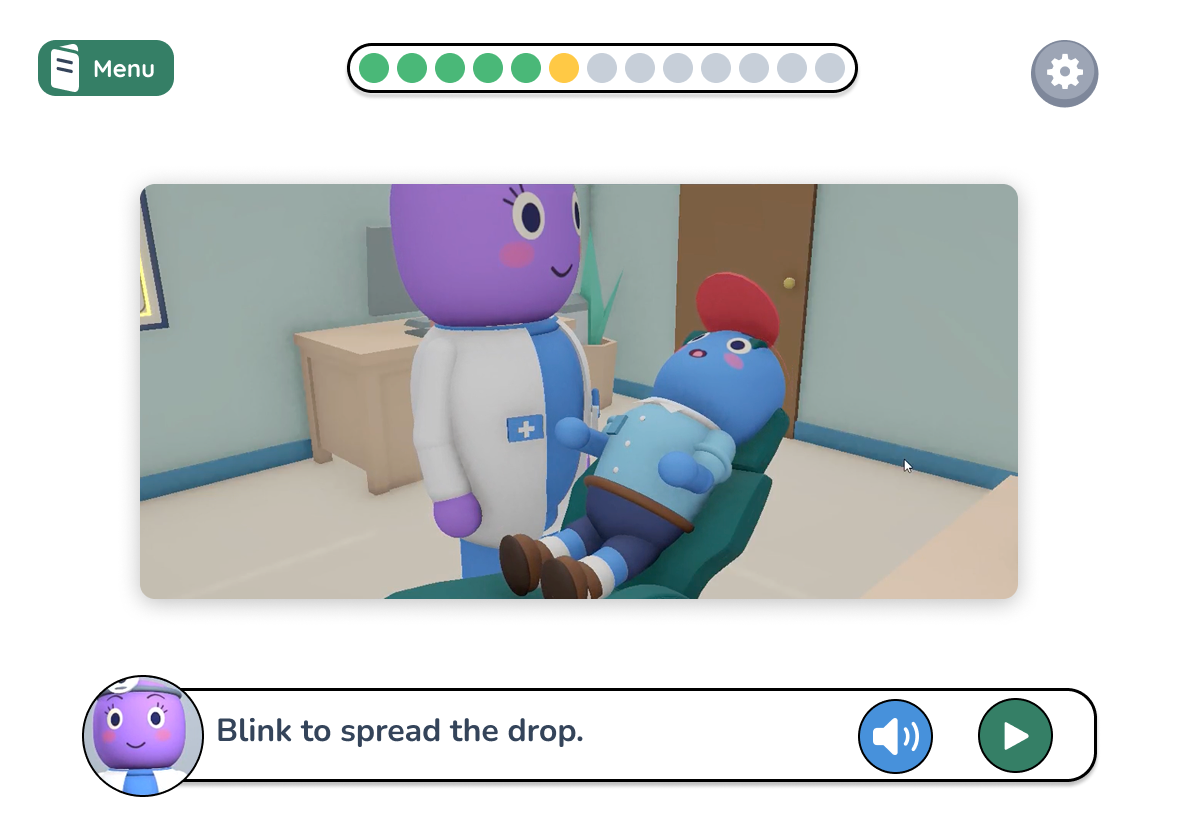
\includegraphics[width=0.8\textwidth]{EyeCanDoCW/Sixth Scene.png}
\end{figure}

\begin{figure}[H]
    \centering
    \caption{Seventh Scene}
    \label{fig:s7}
    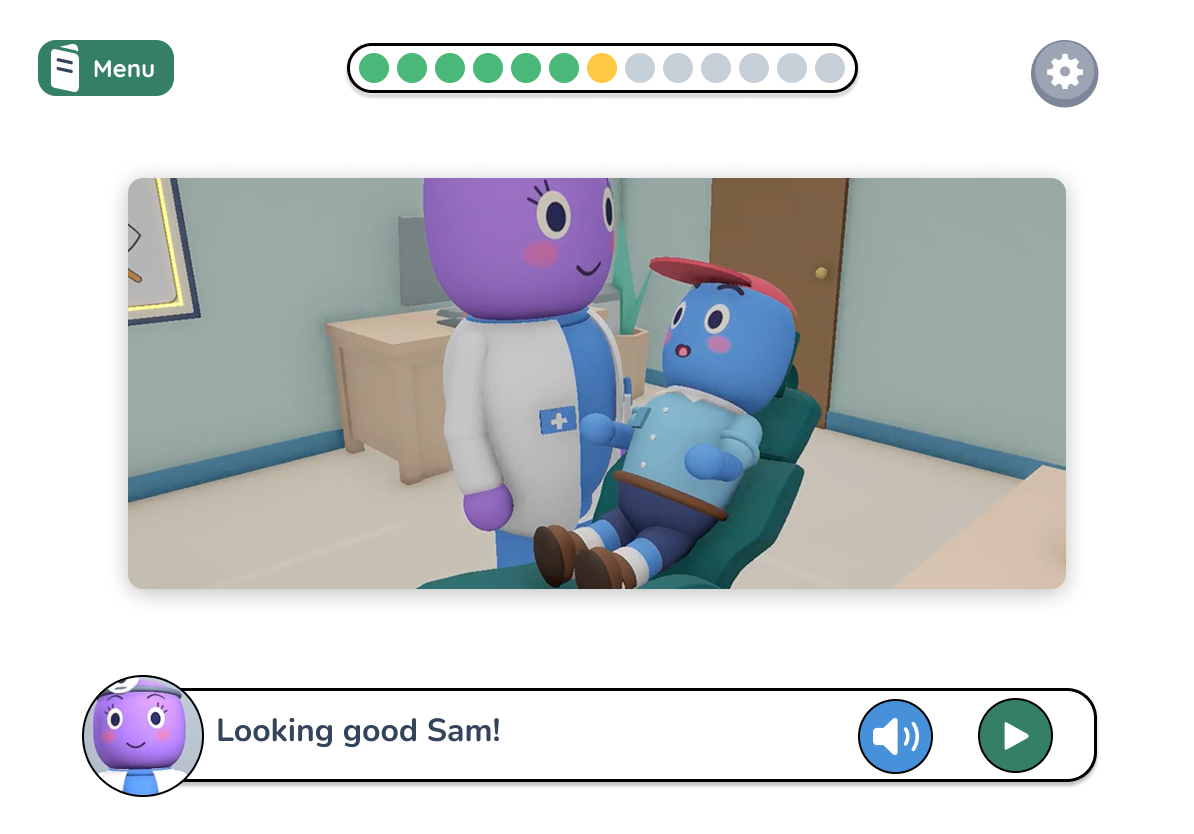
\includegraphics[width=0.8\textwidth]{EyeCanDoCW/Seventh Scene.png}
\end{figure}

\begin{figure}[H]
    \centering
    \caption{Eighth Scene}
    \label{fig:s8}
    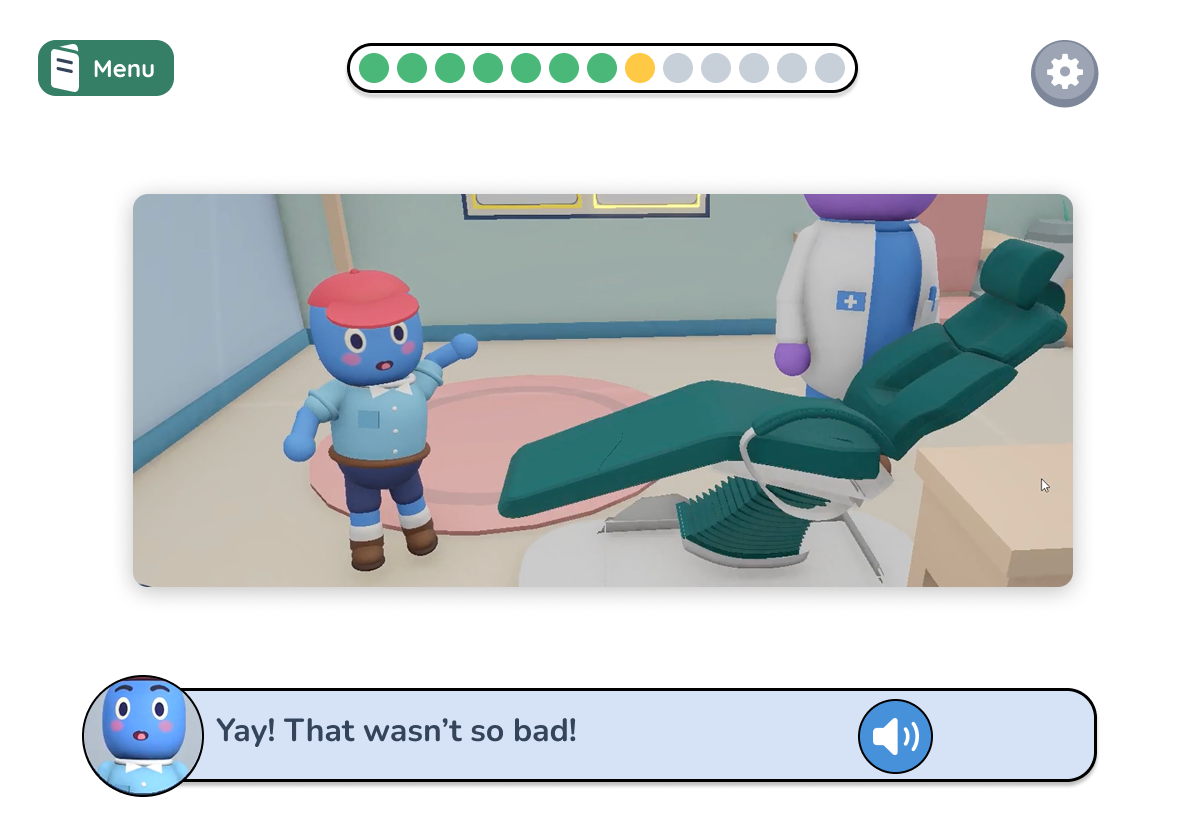
\includegraphics[width=0.8\textwidth]{EyeCanDoCW/Eighth Scene.png}
\end{figure}

\begin{figure}[H]
    \centering
    \caption{Ninth Scene}
    \label{fig:s9}
    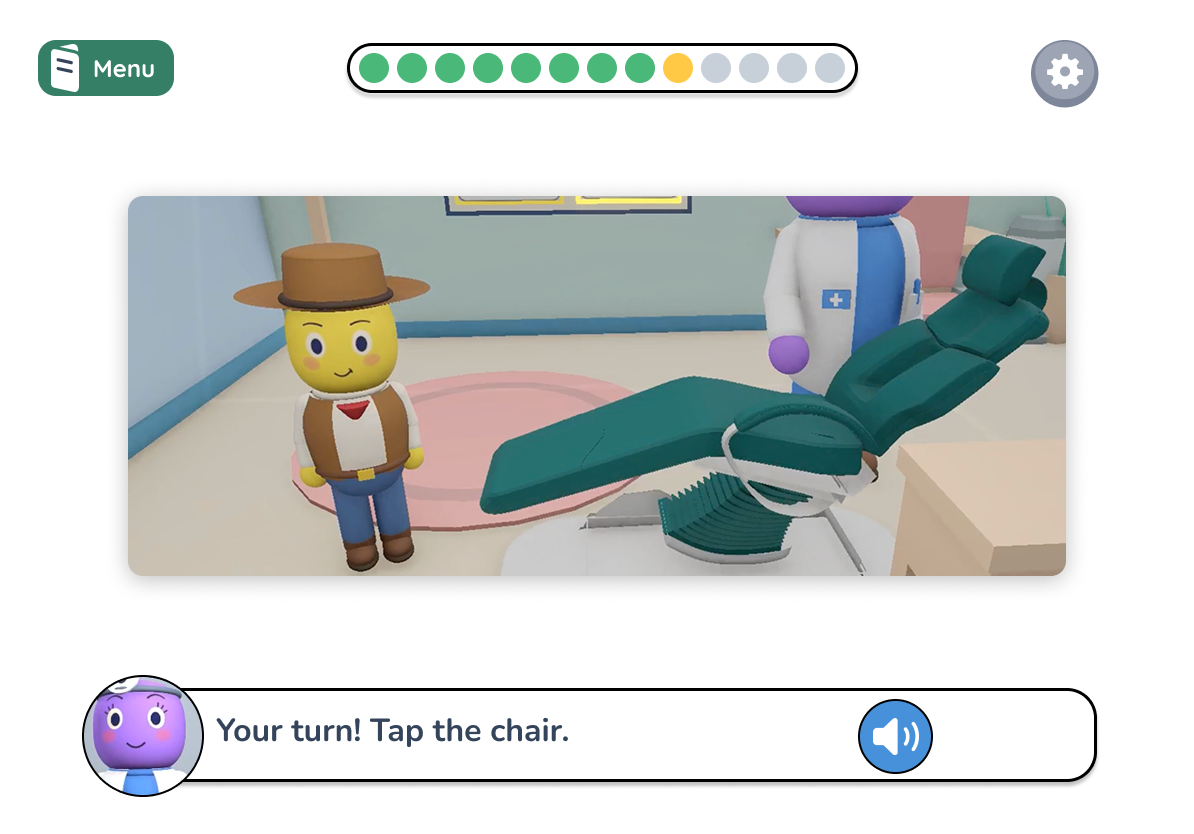
\includegraphics[width=0.8\textwidth]{EyeCanDoCW/Ninth Scene.png}
\end{figure}

\begin{figure}[H]
    \centering
    \caption{Tenth Scene 1}
    \label{fig:s10a}
    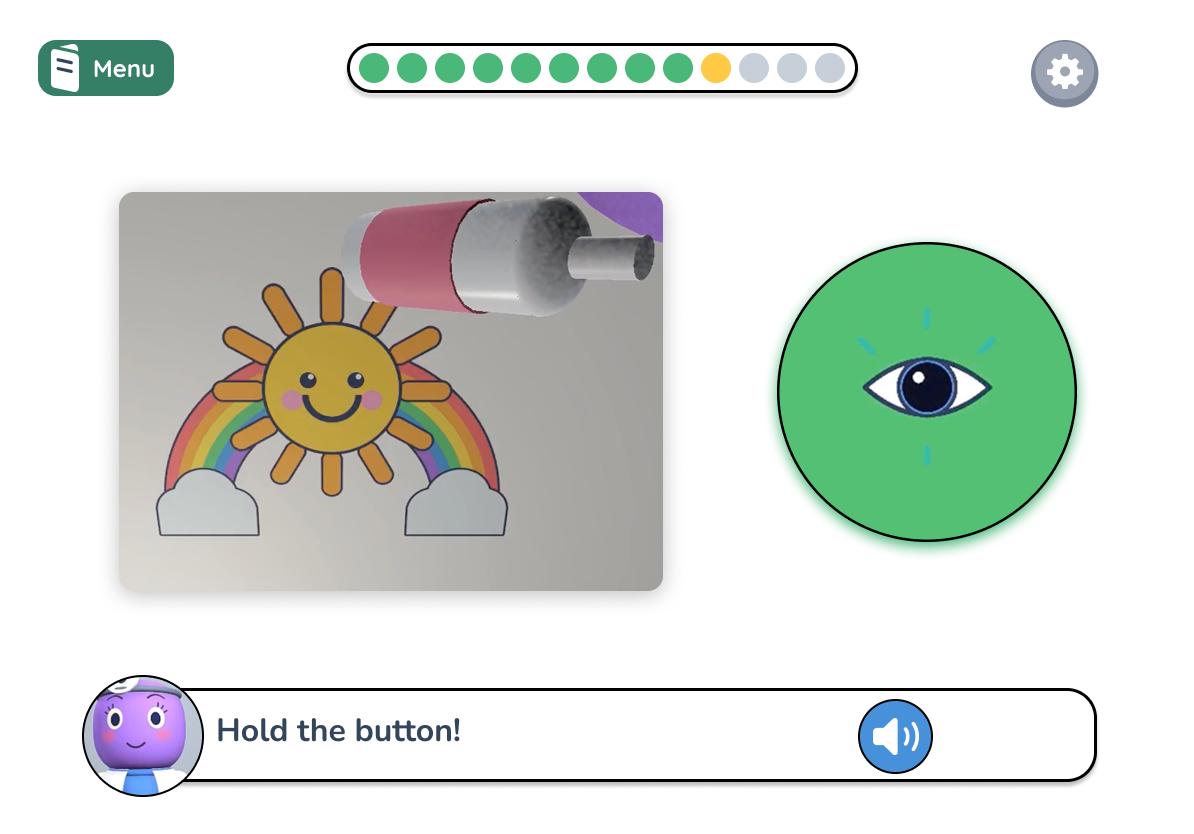
\includegraphics[width=0.8\textwidth]{EyeCanDoCW/Tenth Scene 1.png}
\end{figure}

\begin{figure}[H]
    \centering
    \caption{Tenth Scene 2}
    \label{fig:s10b}
    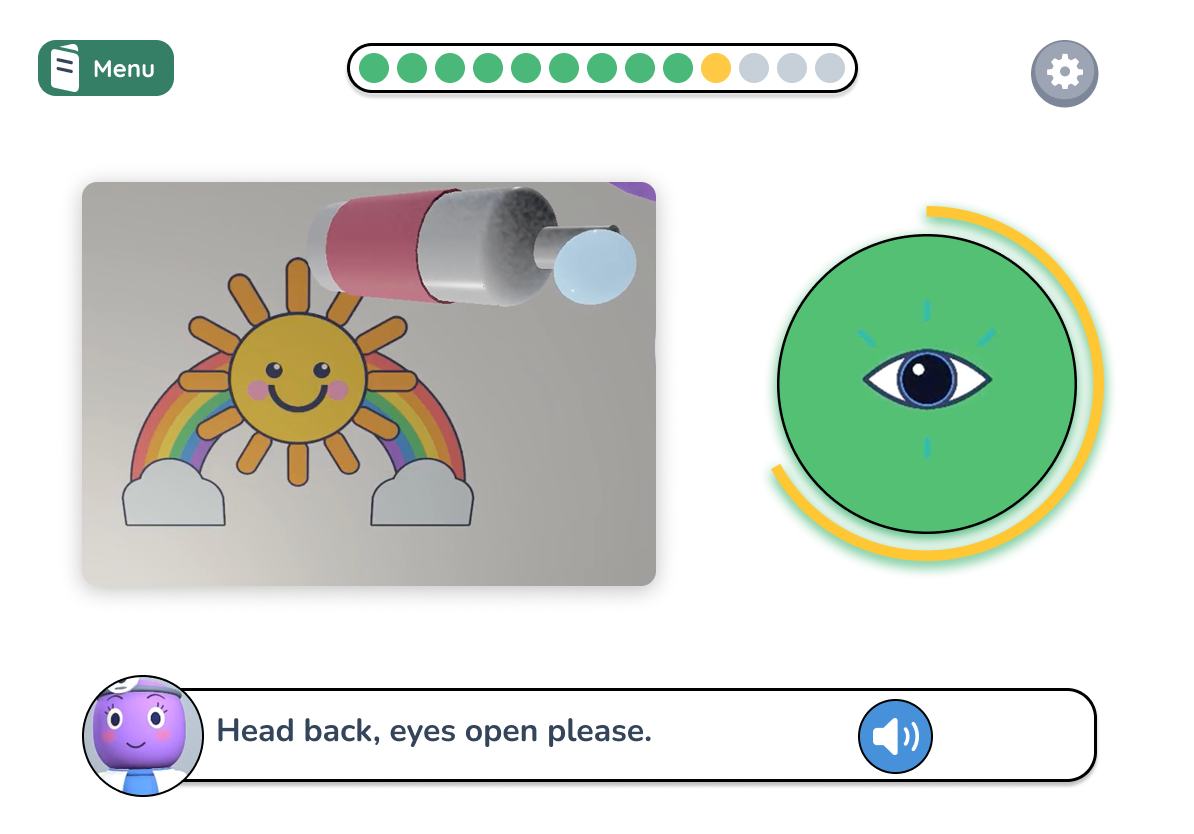
\includegraphics[width=0.8\textwidth]{EyeCanDoCW/Tenth Scene 2.png}
\end{figure}

\begin{figure}[H]
    \centering
    \caption{Eleventh Scene}
    \label{fig:s11}
    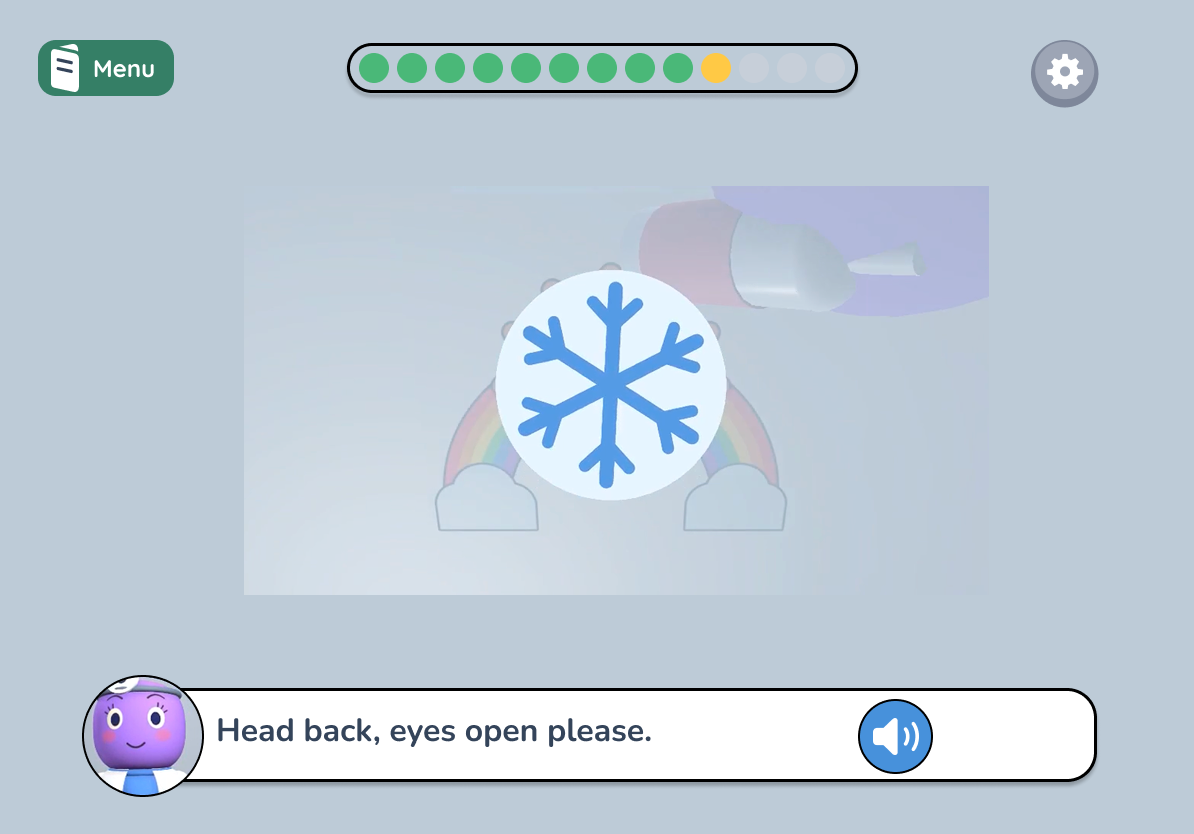
\includegraphics[width=0.8\textwidth]{EyeCanDoCW/EleventhScene.png}
\end{figure}

\begin{figure}[H]
    \centering
    \caption{Twelfth Scene}
    \label{fig:s12a}
    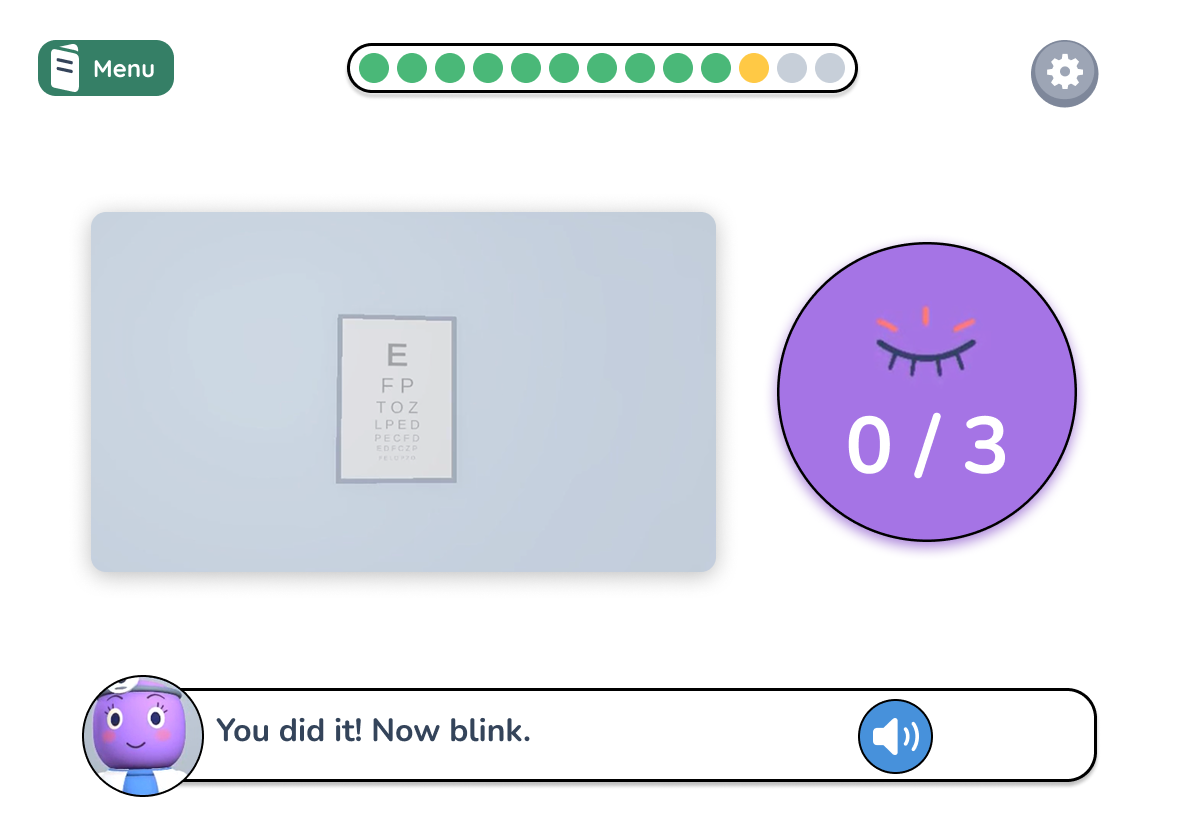
\includegraphics[width=0.8\textwidth]{EyeCanDoCW/Twelfth Scene.png}
\end{figure}

\begin{figure}[H]
    \centering
    \caption{Twelfth Scene 2}
    \label{fig:s12b}
    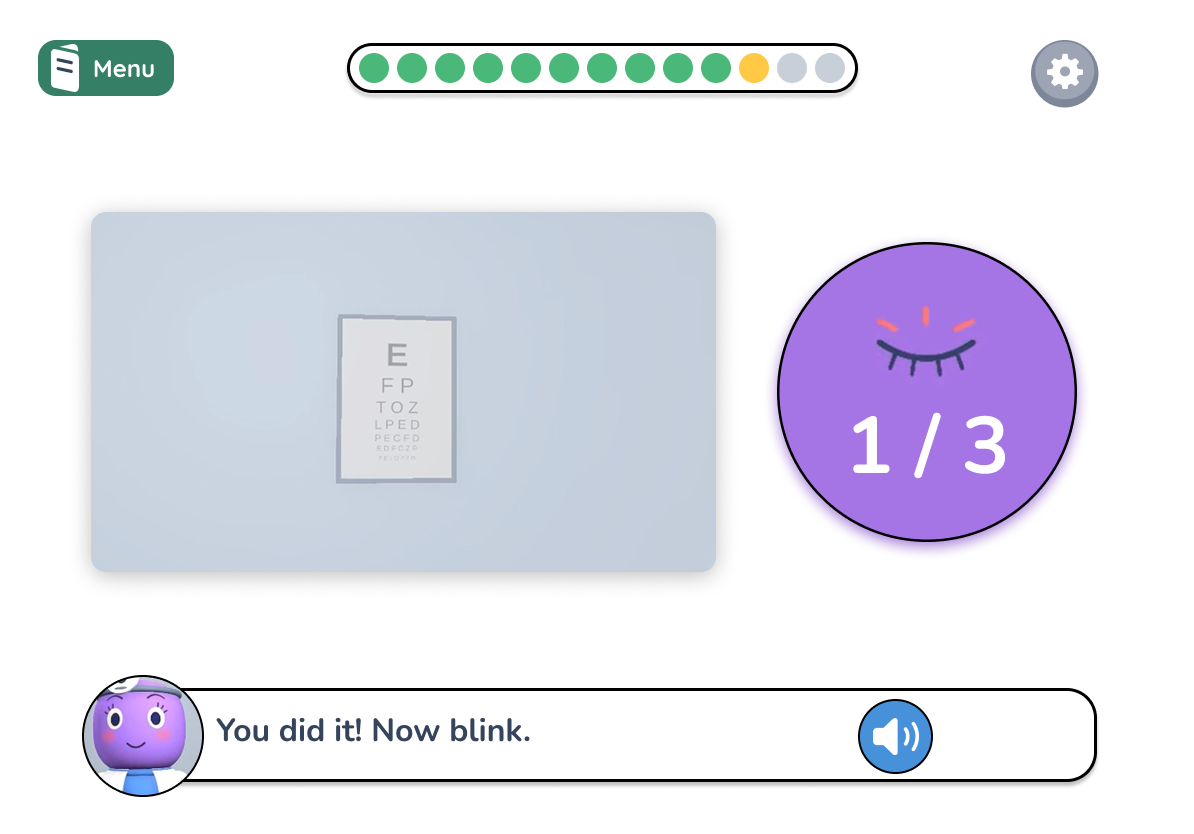
\includegraphics[width=0.8\textwidth]{EyeCanDoCW/Twelfth Scene 2.png}
\end{figure}

\begin{figure}[H]
    \centering
    \caption{Twelfth Scene 3}
    \label{fig:s12c}
    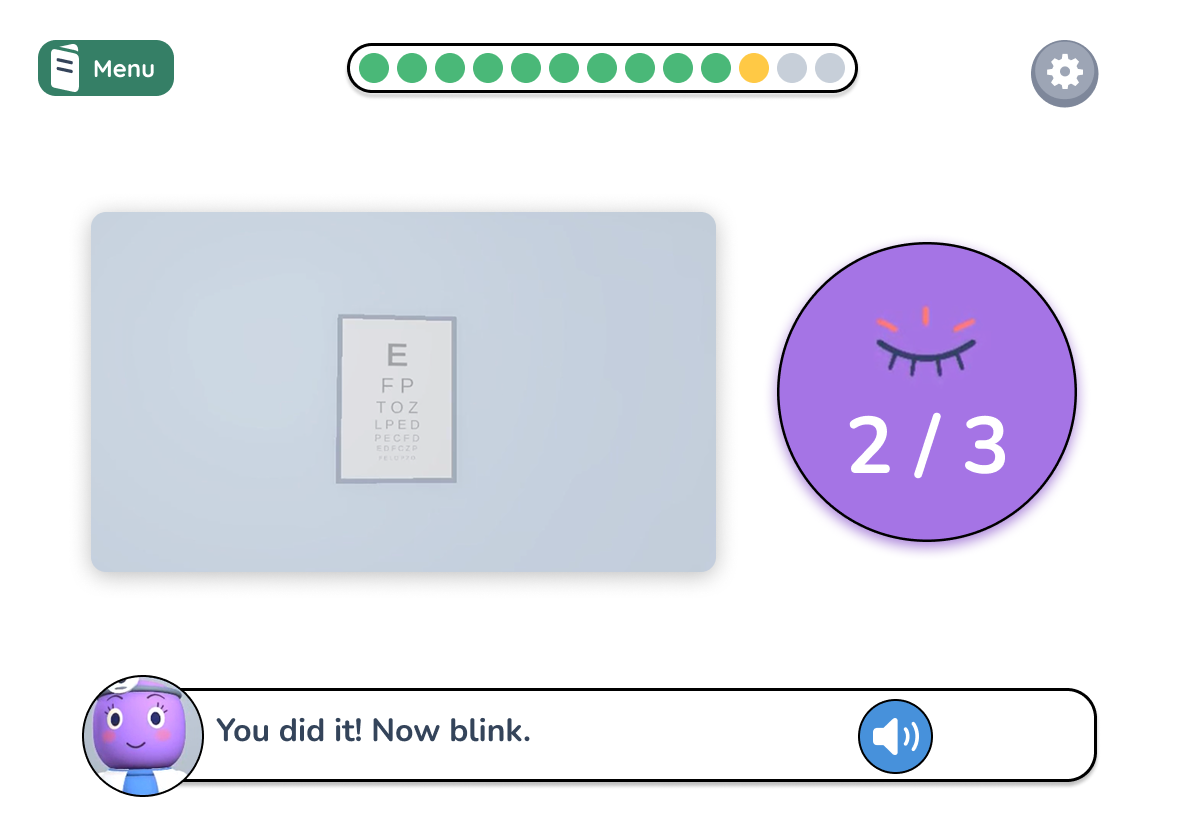
\includegraphics[width=0.8\textwidth]{EyeCanDoCW/Twelfth Scene 3.png}
\end{figure}

\begin{figure}[H]
    \centering
    \caption{Twelfth Scene 4}
    \label{fig:s12d}
    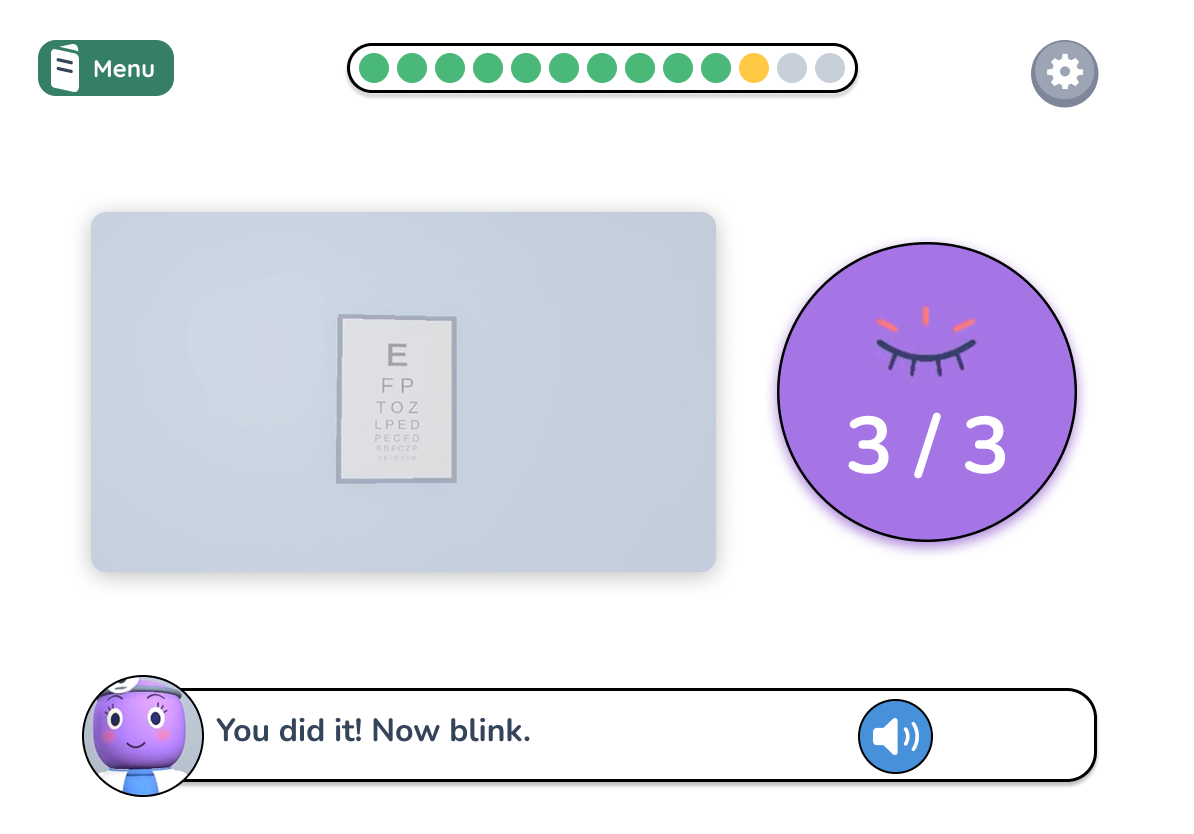
\includegraphics[width=0.8\textwidth]{EyeCanDoCW/Twelfth Scene 4.png}
\end{figure}

\begin{figure}[H]
    \centering
    \caption{Thirteenth Scene}
    \label{fig:s13}
    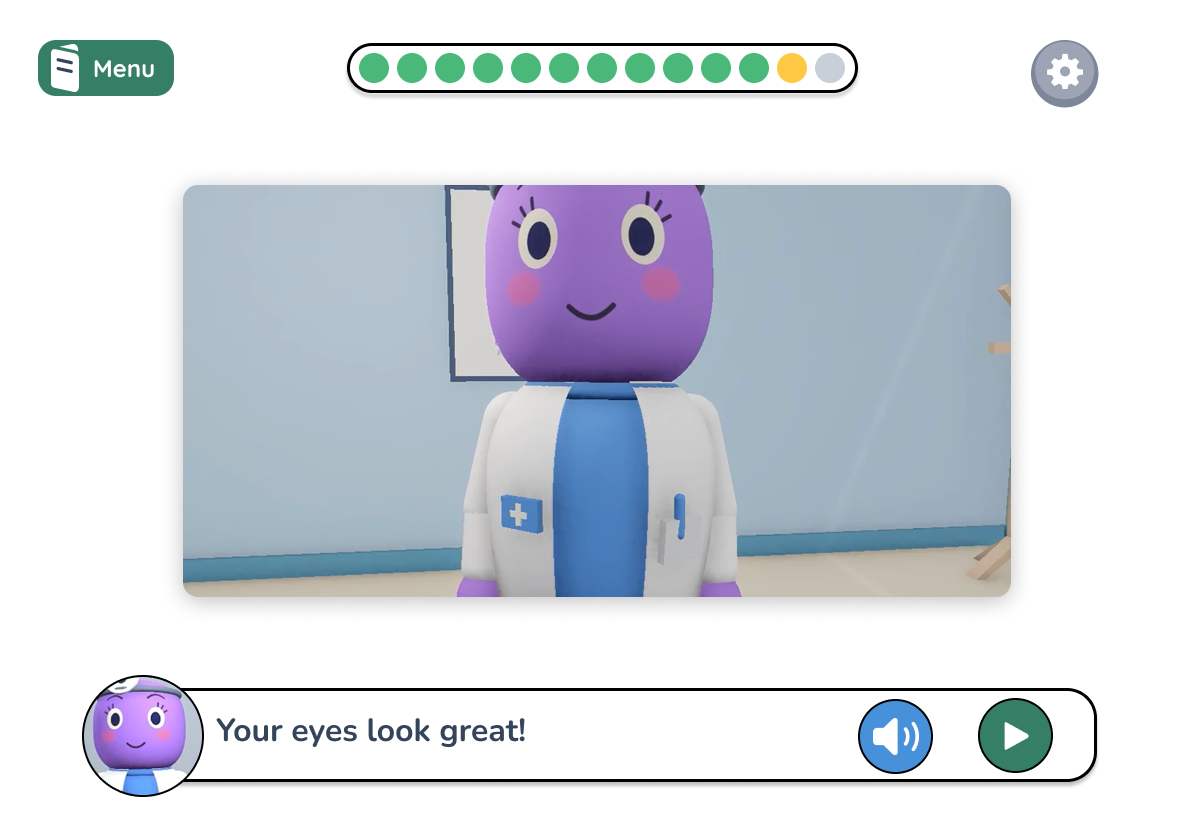
\includegraphics[width=0.8\textwidth]{EyeCanDoCW/Thirteen Scene.png}
\end{figure}

\begin{figure}[H]
    \centering
    \caption{Final Scene 1}
    \label{fig:final1}
    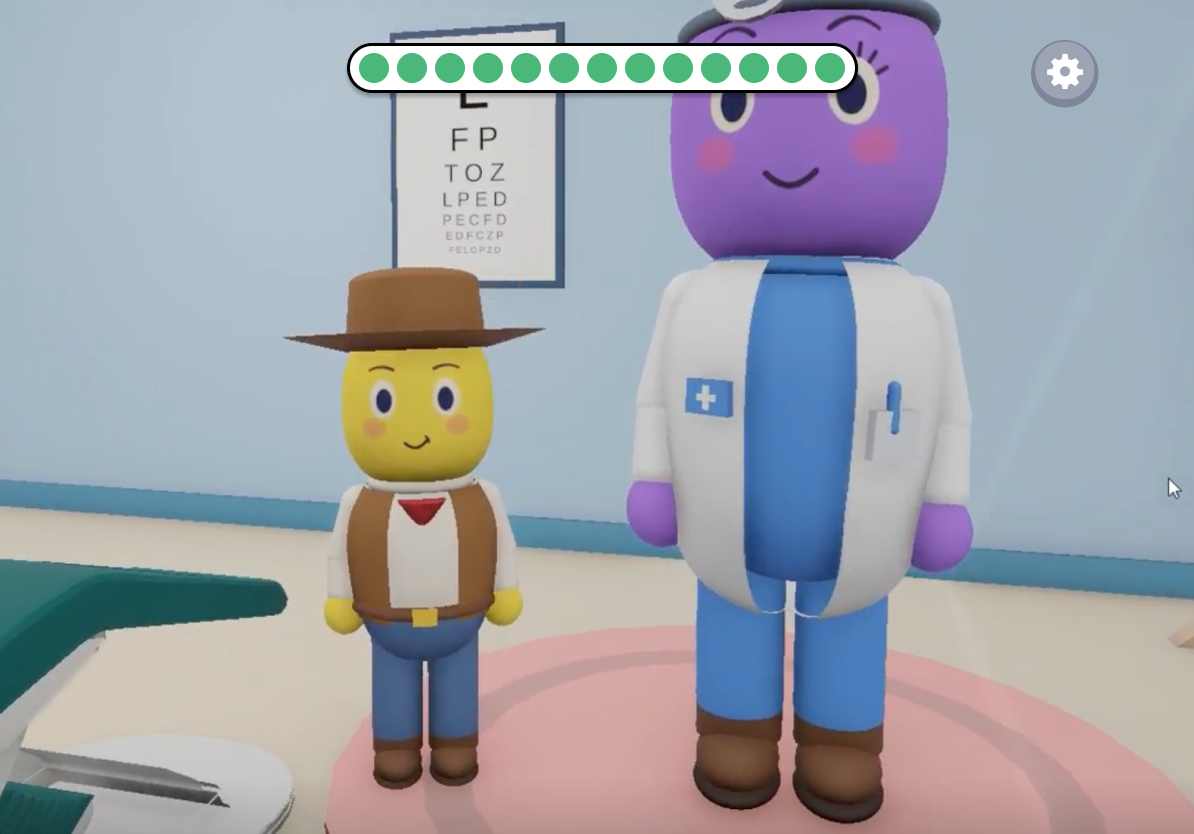
\includegraphics[width=0.8\textwidth]{EyeCanDoCW/Final Scene 1.png}
\end{figure}

\begin{figure}[H]
    \centering
    \caption{Final Scene 2}
    \label{fig:final2}
    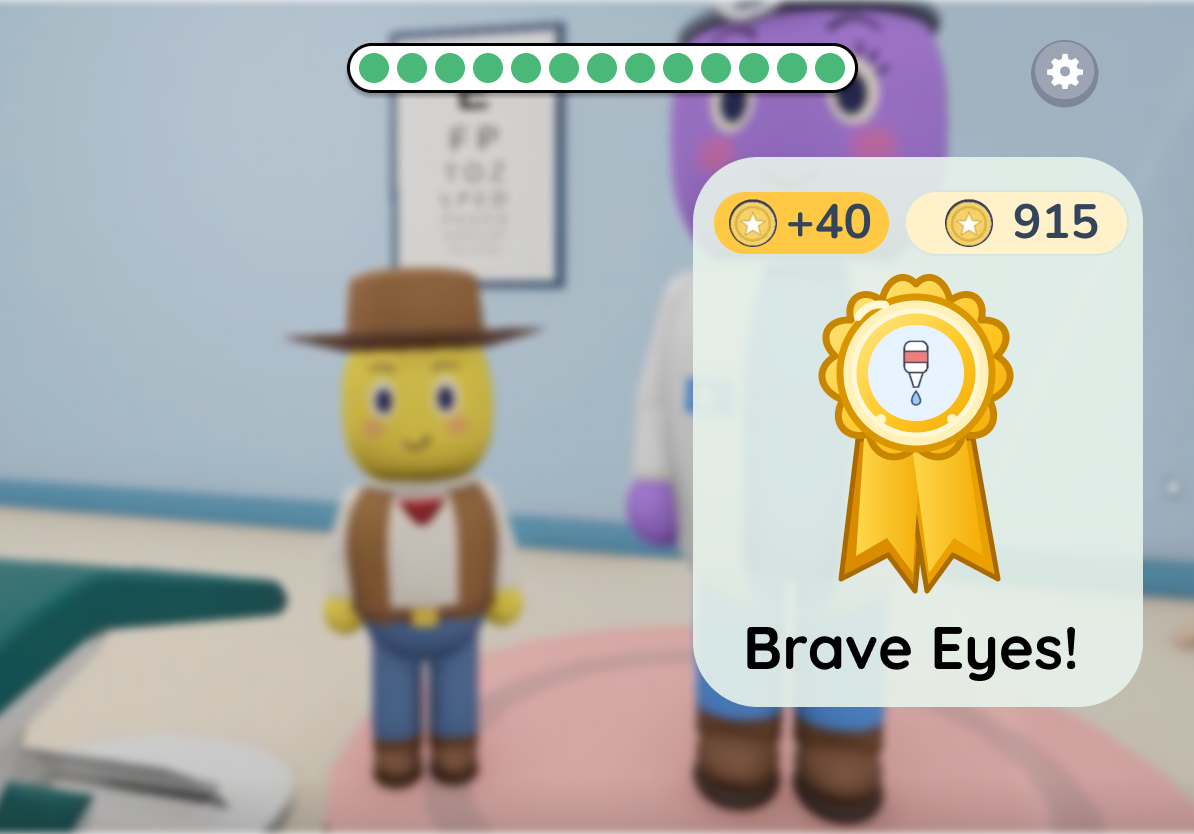
\includegraphics[width=0.8\textwidth]{EyeCanDoCW/Final Scene 2.png}
\end{figure}

\begin{figure}[H]
    \centering
    \caption{Final Scene 3}
    \label{fig:final3}
    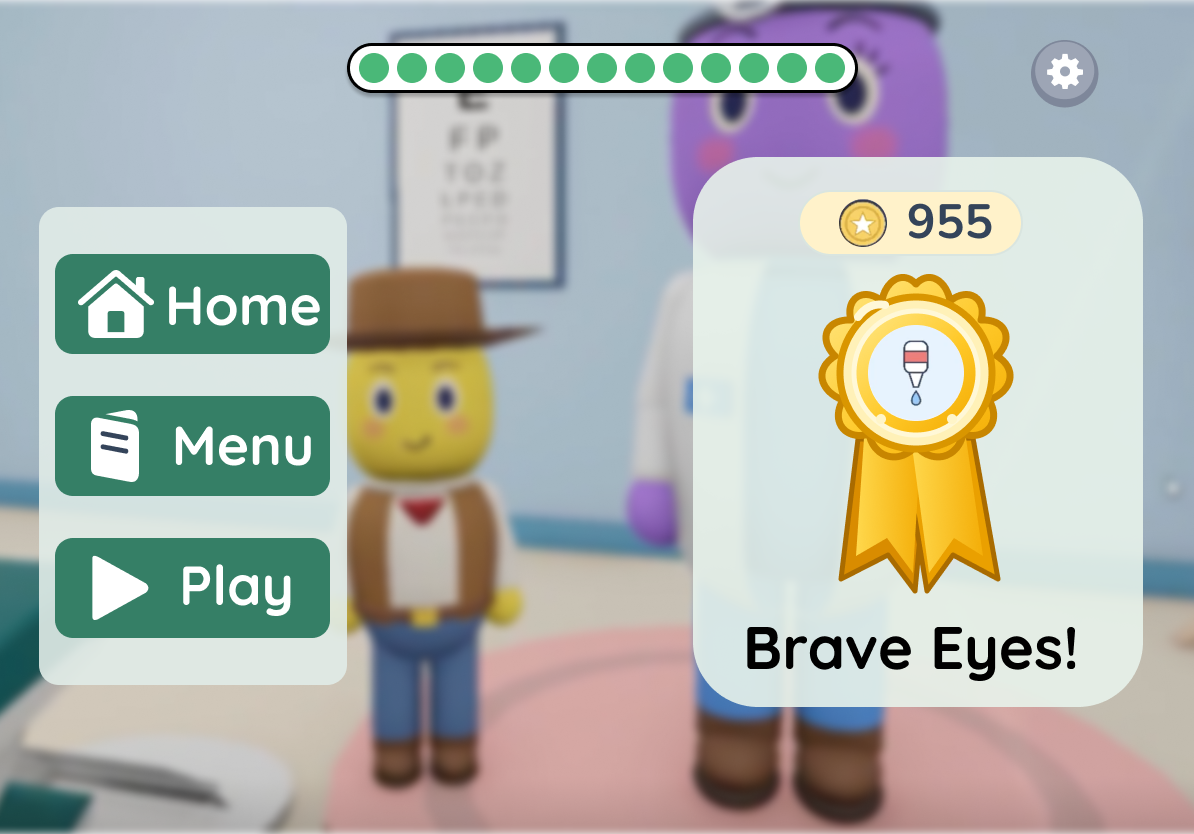
\includegraphics[width=0.8\textwidth]{EyeCanDoCW/Final Scene 3.png}
\end{figure}

\begin{figure}[H]
    \centering
    \caption{Dress Up Fits Scene}
    \label{fig:dressfits}
    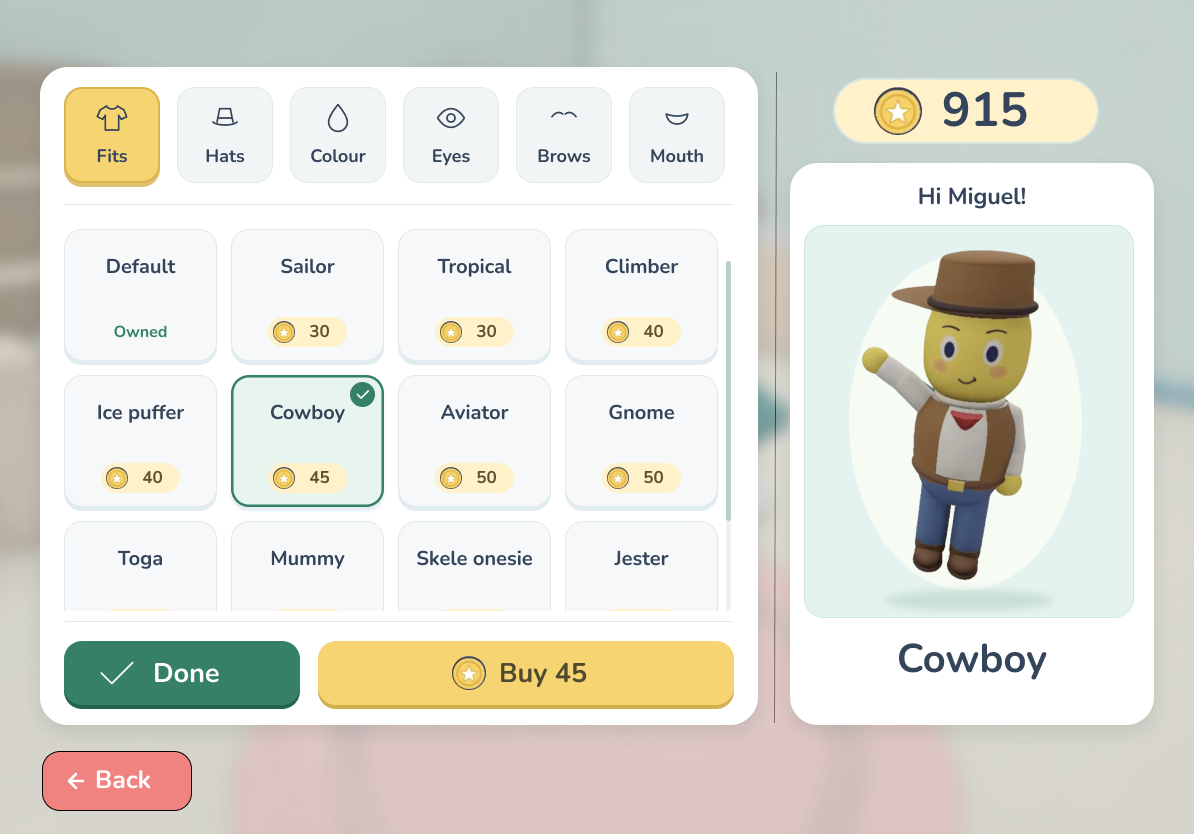
\includegraphics[width=0.8\textwidth]{EyeCanDoCW/Dress Up Fits.png}
\end{figure}

\begin{figure}[H]
    \centering
    \caption{Dress Up Eyes Scene}
    \label{fig:dresseyes}
    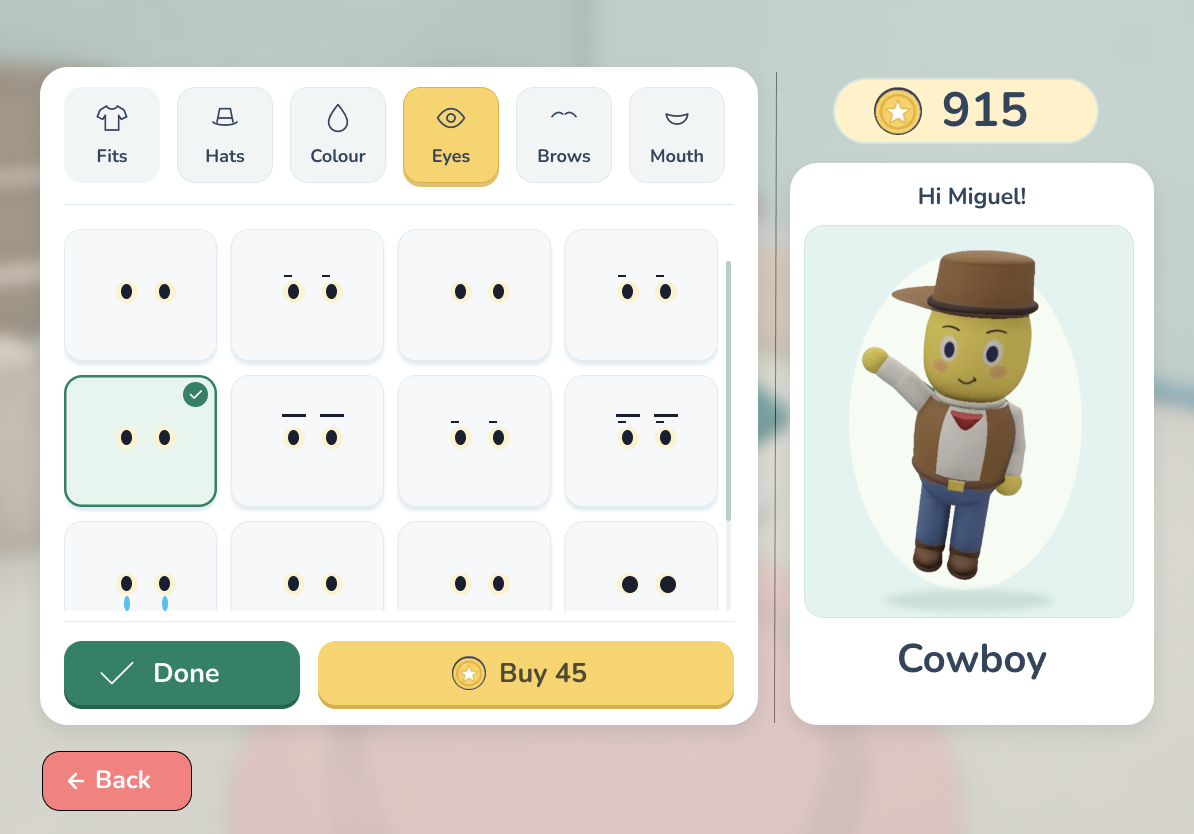
\includegraphics[width=0.8\textwidth]{EyeCanDoCW/Dress Up Eyes.png}
\end{figure}

\newpage

% =====================================================================
\subsection{Appendix B: Generative AI Disclosure}
% =====================================================================

\subsubsection{AI Tools Used}

\begin{itemize}
    \item Claude (Opus 5.5), ChatGPT (Sonnet 5.5)
\end{itemize}

\subsubsection{How and Where Used}

Claude was used as the supporting tool during the preparation of
this document, primarily to assist with \LaTeX{} formatting,
improving wording and clarity, organizing information, and performing 
draft summaries of the collected notes.
They were used in the following sections:

\begin{itemize}
    \item In Section~\ref{sec:intro} Opus was used to create a draft from 
    the resources provided and clarifications given. This was scrutinized 
    and edited to ensure the correct information is presented from the provided
    data and resources.
    \item In Section~\ref{sec:method} Opus was used to create a draft from 
    the resources provided and clarifications given. This was scrutinized 
    and edited to ensure the correct information is presented from the provided
    data and resources. Opus was also used to assist with \LaTeX{} formatting 
    to ensure a good quality document is presented to read.
    \item In Section~\ref{sec:people} Opus was used to assist with \LaTeX{} formatting 
    to ensure a good quality document is presented to read.
    \item In Section~\ref{sec:results} Opus was used to assist with drafting the 
    results and findings by simplifying and cross-referencing the notes with each other.
    The notes were thoroughly reviewed alongside the draft, with multiple fixes occurring 
    to reflect the correct information from the meetings. Opus also helped with 
    \LaTeX{} formatting to ensure a good quality document is presented to read.
    \item In Section~\ref{sec:planned} Opus was used to assist with drafting the 
    of the changes based on the heavily edited results. This was edited thoroughly to 
    reflect the expectations of the team and the requirements in the SRS. Opus also helped with 
    \LaTeX{} formatting to ensure a good quality document is presented to read.
    \item In Section~\ref{sec:figmaPhotos} Opus was used to generate the \LaTeX{} code for the 
    figures to save time. The output was reviewed to ensure all the Figma photos were present 
    with the correct captions.
    \item Opus was used to generate the BibText references for the References.bib file to
    ensure IEEE standards are followed.
    \item The Figma AI Agent and Sonnet 5.5 Plug-in were used in Figma to develop a few draft 
    scenes (Home, Profile) in Figma to assist with development. These scenes were edited for UI 
    and UX purposes to ensure that the work was aligned with the PoC video shown in the cognitive 
    walkthrough

\end{itemize}

\subsubsection{Verification of AI-Generated Content}

Ethan reviewed AI-assisted material to ensure it was
consistent with the project's scope, existing documentation,
and intended application functionality. Ethan reviewed suggested 
wording, data entities, and recommendation approaches before including 
them in the document. Initial design ideas were also noted as needing 
further feedback from the project supervisors.

AI-assisted \LaTeX{} formatting was checked to ensure
that tables and other document elements were presented
correctly. The team remains responsible for the accuracy,
completeness, consistency, and appropriateness of the
final Custom Document.

\newpage

\bibliographystyle{unsrt}
\bibliography{../../refs/References}

\newpage

\end{document}